\documentclass[twoside]{book}

% Packages required by doxygen
\usepackage{calc}
\usepackage{doxygen}
\usepackage{graphicx}
\usepackage[utf8]{inputenc}
\usepackage{makeidx}
\usepackage{multicol}
\usepackage{multirow}
\usepackage{textcomp}
\usepackage[table]{xcolor}

% Font selection
\usepackage[T1]{fontenc}
\usepackage{mathptmx}
\usepackage[scaled=.90]{helvet}
\usepackage{courier}
\usepackage{amssymb}
\usepackage{sectsty}
\renewcommand{\familydefault}{\sfdefault}
\allsectionsfont{%
  \fontseries{bc}\selectfont%
  \color{darkgray}%
}
\renewcommand{\DoxyLabelFont}{%
  \fontseries{bc}\selectfont%
  \color{darkgray}%
}

% Page & text layout
\usepackage{geometry}
\geometry{%
  a4paper,%
  top=2.5cm,%
  bottom=2.5cm,%
  left=2.5cm,%
  right=2.5cm%
}
\tolerance=750
\hfuzz=15pt
\hbadness=750
\setlength{\emergencystretch}{15pt}
\setlength{\parindent}{0cm}
\setlength{\parskip}{0.2cm}
\makeatletter
\renewcommand{\paragraph}{%
  \@startsection{paragraph}{4}{0ex}{-1.0ex}{1.0ex}{%
    \normalfont\normalsize\bfseries\SS@parafont%
  }%
}
\renewcommand{\subparagraph}{%
  \@startsection{subparagraph}{5}{0ex}{-1.0ex}{1.0ex}{%
    \normalfont\normalsize\bfseries\SS@subparafont%
  }%
}
\makeatother

% Headers & footers
\usepackage{fancyhdr}
\pagestyle{fancyplain}
\fancyhead[LE]{\fancyplain{}{\bfseries\thepage}}
\fancyhead[CE]{\fancyplain{}{}}
\fancyhead[RE]{\fancyplain{}{\bfseries\leftmark}}
\fancyhead[LO]{\fancyplain{}{\bfseries\rightmark}}
\fancyhead[CO]{\fancyplain{}{}}
\fancyhead[RO]{\fancyplain{}{\bfseries\thepage}}
\fancyfoot[LE]{\fancyplain{}{}}
\fancyfoot[CE]{\fancyplain{}{}}
\fancyfoot[RE]{\fancyplain{}{\bfseries\scriptsize Generated on Sun Sep 8 2013 08\-:52\-:31 for Tea Tank Library by Doxygen }}
\fancyfoot[LO]{\fancyplain{}{\bfseries\scriptsize Generated on Sun Sep 8 2013 08\-:52\-:31 for Tea Tank Library by Doxygen }}
\fancyfoot[CO]{\fancyplain{}{}}
\fancyfoot[RO]{\fancyplain{}{}}
\renewcommand{\footrulewidth}{0.4pt}
\renewcommand{\chaptermark}[1]{%
  \markboth{#1}{}%
}
\renewcommand{\sectionmark}[1]{%
  \markright{\thesection\ #1}%
}

% Indices & bibliography
\usepackage{natbib}
\usepackage[titles]{tocloft}
\setcounter{tocdepth}{3}
\setcounter{secnumdepth}{5}
\makeindex

% Hyperlinks (required, but should be loaded last)
\usepackage{ifpdf}
\ifpdf
  \usepackage[pdftex,pagebackref=true]{hyperref}
\else
  \usepackage[ps2pdf,pagebackref=true]{hyperref}
\fi
\hypersetup{%
  colorlinks=true,%
  linkcolor=blue,%
  citecolor=blue,%
  unicode%
}

% Custom commands
\newcommand{\clearemptydoublepage}{%
  \newpage{\pagestyle{empty}\cleardoublepage}%
}


%===== C O N T E N T S =====

\begin{document}

% Titlepage & ToC
\hypersetup{pageanchor=false}
\pagenumbering{roman}
\begin{titlepage}
\vspace*{7cm}
\begin{center}%
{\Large Tea Tank Library \\[1ex]\large 2 }\\
\vspace*{1cm}
{\large Generated by Doxygen 1.8.5}\\
\vspace*{0.5cm}
{\small Sun Sep 8 2013 08:52:31}\\
\end{center}
\end{titlepage}
\clearemptydoublepage
\tableofcontents
\clearemptydoublepage
\pagenumbering{arabic}
\hypersetup{pageanchor=true}

%--- Begin generated contents ---
\chapter{Hierarchical Index}
\section{Class Hierarchy}
This inheritance list is sorted roughly, but not completely, alphabetically\-:\begin{DoxyCompactList}
\item \contentsline{section}{ttl\-:\-:Benchmark}{\pageref{classttl_1_1_benchmark}}{}
\item \contentsline{section}{Benchmark}{\pageref{class_benchmark}}{}
\item \contentsline{section}{ttl\-:\-:Flare}{\pageref{classttl_1_1_flare}}{}
\item \contentsline{section}{Flare}{\pageref{class_flare}}{}
\item \contentsline{section}{Ips}{\pageref{class_ips}}{}
\item \contentsline{section}{ttl\-:\-:Ips}{\pageref{classttl_1_1_ips}}{}
\item \contentsline{section}{Join\-Thread}{\pageref{class_join_thread}}{}
\item \contentsline{section}{ttl\-:\-:Logger$<$ State $>$}{\pageref{classttl_1_1_logger}}{}
\item \contentsline{section}{Logger}{\pageref{class_logger}}{}
\item \contentsline{section}{ttl\-:\-:Logger$<$ false $>$}{\pageref{classttl_1_1_logger_3_01false_01_4}}{}
\item \contentsline{section}{ttl\-:\-:Logger$<$ true $>$}{\pageref{classttl_1_1_logger_3_01true_01_4}}{}
\item \contentsline{section}{ttl\-:\-:m\-\_\-\-Timestamp}{\pageref{structttl_1_1m___timestamp}}{}
\item \contentsline{section}{ttl\-:\-:Runnable}{\pageref{classttl_1_1_runnable}}{}
\item \contentsline{section}{ttl\-:\-:Scoped\-Function}{\pageref{classttl_1_1_scoped_function}}{}
\item \contentsline{section}{ttl\-:\-:Synched$<$ T $>$}{\pageref{classttl_1_1_synched}}{}
\item \contentsline{section}{Synched}{\pageref{class_synched}}{}
\item \contentsline{section}{ttl\-:\-:Synched\-Data}{\pageref{structttl_1_1_synched_data}}{}
\item \contentsline{section}{ttl\-:\-:Synched\-Reader$<$ T $>$}{\pageref{classttl_1_1_synched_reader}}{}
\item \contentsline{section}{ttl\-:\-:Synched\-Writer$<$ T $>$}{\pageref{classttl_1_1_synched_writer}}{}
\item thread\begin{DoxyCompactList}
\item \contentsline{section}{ttl\-:\-:Join\-Thread}{\pageref{classttl_1_1_join_thread}}{}
\end{DoxyCompactList}
\item \contentsline{section}{ttl\-:\-:Valman}{\pageref{classttl_1_1_valman}}{}
\item \contentsline{section}{Valman}{\pageref{class_valman}}{}
\item C\-L\-A\-S\-S\-E\-S\begin{DoxyCompactList}
\item \contentsline{section}{ttl\-:\-:Mixin$<$ C\-L\-A\-S\-S\-E\-S $>$}{\pageref{classttl_1_1_mixin}}{}
\end{DoxyCompactList}
\end{DoxyCompactList}

\chapter{Class Index}
\section{Class List}
Here are the classes, structs, unions and interfaces with brief descriptions\-:\begin{DoxyCompactList}
\item\contentsline{section}{\hyperlink{classttl_1_1_benchmark}{ttl\-::\-Benchmark} \\*A benchmarking class }{\pageref{classttl_1_1_benchmark}}{}
\item\contentsline{section}{\hyperlink{class_benchmark}{Benchmark} }{\pageref{class_benchmark}}{}
\item\contentsline{section}{\hyperlink{classttl_1_1_flare}{ttl\-::\-Flare} \\*Simple signalling between threads }{\pageref{classttl_1_1_flare}}{}
\item\contentsline{section}{\hyperlink{class_flare}{Flare} }{\pageref{class_flare}}{}
\item\contentsline{section}{\hyperlink{class_ips}{Ips} }{\pageref{class_ips}}{}
\item\contentsline{section}{\hyperlink{classttl_1_1_ips}{ttl\-::\-Ips} \\*Iteration limiter }{\pageref{classttl_1_1_ips}}{}
\item\contentsline{section}{\hyperlink{classttl_1_1_join_thread}{ttl\-::\-Join\-Thread} \\*Scoped thread that joins at scope exit }{\pageref{classttl_1_1_join_thread}}{}
\item\contentsline{section}{\hyperlink{class_join_thread}{Join\-Thread} }{\pageref{class_join_thread}}{}
\item\contentsline{section}{\hyperlink{classttl_1_1_logger}{ttl\-::\-Logger$<$ State $>$} \\*Simple logging utility }{\pageref{classttl_1_1_logger}}{}
\item\contentsline{section}{\hyperlink{class_logger}{Logger} }{\pageref{class_logger}}{}
\item\contentsline{section}{\hyperlink{classttl_1_1_logger_3_01false_01_4}{ttl\-::\-Logger$<$ false $>$} \\*Simple logging utility -\/ False part }{\pageref{classttl_1_1_logger_3_01false_01_4}}{}
\item\contentsline{section}{\hyperlink{classttl_1_1_logger_3_01true_01_4}{ttl\-::\-Logger$<$ true $>$} \\*Simple logging utility -\/ True part }{\pageref{classttl_1_1_logger_3_01true_01_4}}{}
\item\contentsline{section}{\hyperlink{structttl_1_1m___timestamp}{ttl\-::m\-\_\-\-Timestamp} \\*Dummy variable used in \hyperlink{classttl_1_1_logger}{Logger} for overloads }{\pageref{structttl_1_1m___timestamp}}{}
\item\contentsline{section}{\hyperlink{classttl_1_1_mixin}{ttl\-::\-Mixin$<$ C\-L\-A\-S\-S\-E\-S $>$} \\*A class for mixing classes with eachother }{\pageref{classttl_1_1_mixin}}{}
\item\contentsline{section}{\hyperlink{classttl_1_1_runnable}{ttl\-::\-Runnable} \\*Class for managing cycles of runnable objects }{\pageref{classttl_1_1_runnable}}{}
\item\contentsline{section}{\hyperlink{classttl_1_1_scoped_function}{ttl\-::\-Scoped\-Function} \\*Executes the function upon scope exit }{\pageref{classttl_1_1_scoped_function}}{}
\item\contentsline{section}{\hyperlink{classttl_1_1_synched}{ttl\-::\-Synched$<$ T $>$} \\*Encapsulator that makes objects thread safe }{\pageref{classttl_1_1_synched}}{}
\item\contentsline{section}{\hyperlink{class_synched}{Synched} }{\pageref{class_synched}}{}
\item\contentsline{section}{\hyperlink{structttl_1_1_synched_data}{ttl\-::\-Synched\-Data} \\*Wrapper of \hyperlink{classttl_1_1_synched}{Synched}'s internal data }{\pageref{structttl_1_1_synched_data}}{}
\item\contentsline{section}{\hyperlink{classttl_1_1_synched_reader}{ttl\-::\-Synched\-Reader$<$ T $>$} \\*The reader object }{\pageref{classttl_1_1_synched_reader}}{}
\item\contentsline{section}{\hyperlink{classttl_1_1_synched_writer}{ttl\-::\-Synched\-Writer$<$ T $>$} \\*The writer object }{\pageref{classttl_1_1_synched_writer}}{}
\item\contentsline{section}{\hyperlink{classttl_1_1_valman}{ttl\-::\-Valman} \\*Value manager and loader }{\pageref{classttl_1_1_valman}}{}
\item\contentsline{section}{\hyperlink{class_valman}{Valman} }{\pageref{class_valman}}{}
\end{DoxyCompactList}

\chapter{Class Documentation}
\hypertarget{classttl_1_1_benchmark}{\section{ttl\-:\-:Benchmark Class Reference}
\label{classttl_1_1_benchmark}\index{ttl\-::\-Benchmark@{ttl\-::\-Benchmark}}
}


A benchmarking class.  




{\ttfamily \#include $<$Benchmark.\-hpp$>$}

\subsection*{Public Member Functions}
\begin{DoxyCompactItemize}
\item 
\hyperlink{classttl_1_1_benchmark_a1a14c33331e9b2e7c328a00088a3f4cf}{Benchmark} (const char $\ast$title=\char`\"{}Unnamed benchmark\char`\"{}, const std\-::size\-\_\-t iterations=1)
\begin{DoxyCompactList}\small\item\em Constructor. \end{DoxyCompactList}\item 
\hyperlink{classttl_1_1_benchmark_abbc410384a29c371b442a74cd9c1e224}{Benchmark} (const std\-::string \&title, const std\-::size\-\_\-t iterations=1)
\begin{DoxyCompactList}\small\item\em Constructor. \end{DoxyCompactList}\item 
\hyperlink{classttl_1_1_benchmark_a9889968c38f3799960ff1ea768511eb7}{Benchmark} (const std\-::size\-\_\-t iterations=1)
\begin{DoxyCompactList}\small\item\em Constructor. \end{DoxyCompactList}\item 
\hyperlink{classttl_1_1_benchmark_a94fa0904de8741737e025b00a44bb78f}{Benchmark} (const \hyperlink{classttl_1_1_benchmark}{Benchmark} \&benchmark)
\begin{DoxyCompactList}\small\item\em Copy constructor. \end{DoxyCompactList}\item 
\hyperlink{classttl_1_1_benchmark_a9b27529d09529960ac86adfd5bd0e1d9}{Benchmark} (\hyperlink{classttl_1_1_benchmark}{Benchmark} \&\&benchmark)
\begin{DoxyCompactList}\small\item\em Move constructor. \end{DoxyCompactList}\item 
\hyperlink{classttl_1_1_benchmark}{Benchmark} \& \hyperlink{classttl_1_1_benchmark_a69ee7dbcce5b20e84531efcb45798b51}{operator=} (const \hyperlink{classttl_1_1_benchmark}{Benchmark} \&benchmark)
\begin{DoxyCompactList}\small\item\em Copy assignment. \end{DoxyCompactList}\item 
\hyperlink{classttl_1_1_benchmark}{Benchmark} \& \hyperlink{classttl_1_1_benchmark_a1d7327984894e6ffce05d70836727e2c}{operator=} (\hyperlink{classttl_1_1_benchmark}{Benchmark} \&\&benchmark)
\begin{DoxyCompactList}\small\item\em Move assignment. \end{DoxyCompactList}\item 
\hypertarget{classttl_1_1_benchmark_a194cd9074f96736102831fa818d890a3}{\hyperlink{classttl_1_1_benchmark_a194cd9074f96736102831fa818d890a3}{$\sim$\-Benchmark} ()}\label{classttl_1_1_benchmark_a194cd9074f96736102831fa818d890a3}

\begin{DoxyCompactList}\small\item\em Destructor. \end{DoxyCompactList}\item 
{\footnotesize template$<$typename... Args$>$ }\\void \hyperlink{classttl_1_1_benchmark_a5739a5a9d2634d4b74676b70166ef9e1}{run} (Args \&\&...args)
\begin{DoxyCompactList}\small\item\em Actual running algorithm. \end{DoxyCompactList}\item 
\hypertarget{classttl_1_1_benchmark_aa24491ab2be4d5d9790883b6c3dde656}{void \hyperlink{classttl_1_1_benchmark_aa24491ab2be4d5d9790883b6c3dde656}{reset\-Average\-Run\-Time} ()}\label{classttl_1_1_benchmark_aa24491ab2be4d5d9790883b6c3dde656}

\begin{DoxyCompactList}\small\item\em Reset the average running time. \end{DoxyCompactList}\item 
\hypertarget{classttl_1_1_benchmark_a8135ff02ee37bf040b7cb10aa949adf7}{void \hyperlink{classttl_1_1_benchmark_a8135ff02ee37bf040b7cb10aa949adf7}{set\-Iterations} (const std\-::size\-\_\-t amount)}\label{classttl_1_1_benchmark_a8135ff02ee37bf040b7cb10aa949adf7}

\begin{DoxyCompactList}\small\item\em Set the amount of iterations per benchmark. \end{DoxyCompactList}\item 
float \hyperlink{classttl_1_1_benchmark_ade766a7dd34bbca7039635818edc5a55}{get\-Average\-Run\-Time} () const 
\begin{DoxyCompactList}\small\item\em Get the average running time per benchmark. \end{DoxyCompactList}\end{DoxyCompactItemize}
\subsection*{Friends}
\begin{DoxyCompactItemize}
\item 
std\-::ostream \& \hyperlink{classttl_1_1_benchmark_a2346a28755599b425b019bbda165f9ac}{operator$<$$<$} (std\-::ostream \&lhs, const \hyperlink{classttl_1_1_benchmark}{Benchmark} \&rhs)
\begin{DoxyCompactList}\small\item\em Overload of the ostream operator. \end{DoxyCompactList}\end{DoxyCompactItemize}


\subsection{Detailed Description}
A benchmarking class. 

A class designed for handling benchmarks of functions. It is possible to use member functions, lambdas, function pointers and const function pointers (normal functions). 

\subsection{Constructor \& Destructor Documentation}
\hypertarget{classttl_1_1_benchmark_a1a14c33331e9b2e7c328a00088a3f4cf}{\index{ttl\-::\-Benchmark@{ttl\-::\-Benchmark}!Benchmark@{Benchmark}}
\index{Benchmark@{Benchmark}!ttl::Benchmark@{ttl\-::\-Benchmark}}
\subsubsection[{Benchmark}]{\setlength{\rightskip}{0pt plus 5cm}ttl\-::\-Benchmark\-::\-Benchmark (
\begin{DoxyParamCaption}
\item[{const char $\ast$}]{title = {\ttfamily \char`\"{}Unnamed~benchmark\char`\"{}}, }
\item[{const std\-::size\-\_\-t}]{iterations = {\ttfamily 1}}
\end{DoxyParamCaption}
)}}\label{classttl_1_1_benchmark_a1a14c33331e9b2e7c328a00088a3f4cf}


Constructor. 


\begin{DoxyParams}{Parameters}
{\em title} & The title to give this benchmark \\
\hline
{\em iterations} & The amount of calls to benchmark \\
\hline
\end{DoxyParams}
\hypertarget{classttl_1_1_benchmark_abbc410384a29c371b442a74cd9c1e224}{\index{ttl\-::\-Benchmark@{ttl\-::\-Benchmark}!Benchmark@{Benchmark}}
\index{Benchmark@{Benchmark}!ttl::Benchmark@{ttl\-::\-Benchmark}}
\subsubsection[{Benchmark}]{\setlength{\rightskip}{0pt plus 5cm}ttl\-::\-Benchmark\-::\-Benchmark (
\begin{DoxyParamCaption}
\item[{const std\-::string \&}]{title, }
\item[{const std\-::size\-\_\-t}]{iterations = {\ttfamily 1}}
\end{DoxyParamCaption}
)\hspace{0.3cm}{\ttfamily [explicit]}}}\label{classttl_1_1_benchmark_abbc410384a29c371b442a74cd9c1e224}


Constructor. 


\begin{DoxyParams}{Parameters}
{\em title} & The title to give this benchmark \\
\hline
{\em iterations} & The amount of calls to benchmark \\
\hline
\end{DoxyParams}
\hypertarget{classttl_1_1_benchmark_a9889968c38f3799960ff1ea768511eb7}{\index{ttl\-::\-Benchmark@{ttl\-::\-Benchmark}!Benchmark@{Benchmark}}
\index{Benchmark@{Benchmark}!ttl::Benchmark@{ttl\-::\-Benchmark}}
\subsubsection[{Benchmark}]{\setlength{\rightskip}{0pt plus 5cm}ttl\-::\-Benchmark\-::\-Benchmark (
\begin{DoxyParamCaption}
\item[{const std\-::size\-\_\-t}]{iterations = {\ttfamily 1}}
\end{DoxyParamCaption}
)}}\label{classttl_1_1_benchmark_a9889968c38f3799960ff1ea768511eb7}


Constructor. 


\begin{DoxyParams}{Parameters}
{\em iterations} & The amount of calls to benchmark \\
\hline
\end{DoxyParams}
\hypertarget{classttl_1_1_benchmark_a94fa0904de8741737e025b00a44bb78f}{\index{ttl\-::\-Benchmark@{ttl\-::\-Benchmark}!Benchmark@{Benchmark}}
\index{Benchmark@{Benchmark}!ttl::Benchmark@{ttl\-::\-Benchmark}}
\subsubsection[{Benchmark}]{\setlength{\rightskip}{0pt plus 5cm}ttl\-::\-Benchmark\-::\-Benchmark (
\begin{DoxyParamCaption}
\item[{const {\bf Benchmark} \&}]{benchmark}
\end{DoxyParamCaption}
)}}\label{classttl_1_1_benchmark_a94fa0904de8741737e025b00a44bb78f}


Copy constructor. 


\begin{DoxyParams}{Parameters}
{\em benchmark} & The benchmark to copy \\
\hline
\end{DoxyParams}
\hypertarget{classttl_1_1_benchmark_a9b27529d09529960ac86adfd5bd0e1d9}{\index{ttl\-::\-Benchmark@{ttl\-::\-Benchmark}!Benchmark@{Benchmark}}
\index{Benchmark@{Benchmark}!ttl::Benchmark@{ttl\-::\-Benchmark}}
\subsubsection[{Benchmark}]{\setlength{\rightskip}{0pt plus 5cm}ttl\-::\-Benchmark\-::\-Benchmark (
\begin{DoxyParamCaption}
\item[{{\bf Benchmark} \&\&}]{benchmark}
\end{DoxyParamCaption}
)}}\label{classttl_1_1_benchmark_a9b27529d09529960ac86adfd5bd0e1d9}


Move constructor. 


\begin{DoxyParams}{Parameters}
{\em benchmark} & The benchmark to move \\
\hline
\end{DoxyParams}


\subsection{Member Function Documentation}
\hypertarget{classttl_1_1_benchmark_ade766a7dd34bbca7039635818edc5a55}{\index{ttl\-::\-Benchmark@{ttl\-::\-Benchmark}!get\-Average\-Run\-Time@{get\-Average\-Run\-Time}}
\index{get\-Average\-Run\-Time@{get\-Average\-Run\-Time}!ttl::Benchmark@{ttl\-::\-Benchmark}}
\subsubsection[{get\-Average\-Run\-Time}]{\setlength{\rightskip}{0pt plus 5cm}float ttl\-::\-Benchmark\-::get\-Average\-Run\-Time (
\begin{DoxyParamCaption}
{}
\end{DoxyParamCaption}
) const}}\label{classttl_1_1_benchmark_ade766a7dd34bbca7039635818edc5a55}


Get the average running time per benchmark. 

\begin{DoxyReturn}{Returns}
the running time in microseconds 
\end{DoxyReturn}
\hypertarget{classttl_1_1_benchmark_a69ee7dbcce5b20e84531efcb45798b51}{\index{ttl\-::\-Benchmark@{ttl\-::\-Benchmark}!operator=@{operator=}}
\index{operator=@{operator=}!ttl::Benchmark@{ttl\-::\-Benchmark}}
\subsubsection[{operator=}]{\setlength{\rightskip}{0pt plus 5cm}{\bf Benchmark}\& ttl\-::\-Benchmark\-::operator= (
\begin{DoxyParamCaption}
\item[{const {\bf Benchmark} \&}]{benchmark}
\end{DoxyParamCaption}
)}}\label{classttl_1_1_benchmark_a69ee7dbcce5b20e84531efcb45798b51}


Copy assignment. 


\begin{DoxyParams}{Parameters}
{\em benchmark} & The benchmark to move \\
\hline
\end{DoxyParams}
\begin{DoxyReturn}{Returns}
A reference to itself 
\end{DoxyReturn}
\hypertarget{classttl_1_1_benchmark_a1d7327984894e6ffce05d70836727e2c}{\index{ttl\-::\-Benchmark@{ttl\-::\-Benchmark}!operator=@{operator=}}
\index{operator=@{operator=}!ttl::Benchmark@{ttl\-::\-Benchmark}}
\subsubsection[{operator=}]{\setlength{\rightskip}{0pt plus 5cm}{\bf Benchmark}\& ttl\-::\-Benchmark\-::operator= (
\begin{DoxyParamCaption}
\item[{{\bf Benchmark} \&\&}]{benchmark}
\end{DoxyParamCaption}
)}}\label{classttl_1_1_benchmark_a1d7327984894e6ffce05d70836727e2c}


Move assignment. 


\begin{DoxyParams}{Parameters}
{\em benchmark} & The benchmark to move \\
\hline
\end{DoxyParams}
\begin{DoxyReturn}{Returns}
A reference to itself 
\end{DoxyReturn}
\hypertarget{classttl_1_1_benchmark_a5739a5a9d2634d4b74676b70166ef9e1}{\index{ttl\-::\-Benchmark@{ttl\-::\-Benchmark}!run@{run}}
\index{run@{run}!ttl::Benchmark@{ttl\-::\-Benchmark}}
\subsubsection[{run}]{\setlength{\rightskip}{0pt plus 5cm}template$<$typename... Args$>$ void ttl\-::\-Benchmark\-::run (
\begin{DoxyParamCaption}
\item[{Args \&\&...}]{args}
\end{DoxyParamCaption}
)\hspace{0.3cm}{\ttfamily [inline]}}}\label{classttl_1_1_benchmark_a5739a5a9d2634d4b74676b70166ef9e1}


Actual running algorithm. 

Will loop over the function n times specified by set\-Iterations or by the constructor. The running time will be added to the old running time and then halfed in order to approximate an average.


\begin{DoxyParams}{Parameters}
{\em args} & first a function and then optional arguments \\
\hline
\end{DoxyParams}


\subsection{Friends And Related Function Documentation}
\hypertarget{classttl_1_1_benchmark_a2346a28755599b425b019bbda165f9ac}{\index{ttl\-::\-Benchmark@{ttl\-::\-Benchmark}!operator$<$$<$@{operator$<$$<$}}
\index{operator$<$$<$@{operator$<$$<$}!ttl::Benchmark@{ttl\-::\-Benchmark}}
\subsubsection[{operator$<$$<$}]{\setlength{\rightskip}{0pt plus 5cm}std\-::ostream\& operator$<$$<$ (
\begin{DoxyParamCaption}
\item[{std\-::ostream \&}]{lhs, }
\item[{const {\bf Benchmark} \&}]{rhs}
\end{DoxyParamCaption}
)\hspace{0.3cm}{\ttfamily [friend]}}}\label{classttl_1_1_benchmark_a2346a28755599b425b019bbda165f9ac}


Overload of the ostream operator. 

Outputs the name of the benchmark and the time cost per iteration.


\begin{DoxyParams}{Parameters}
{\em lhs} & the stream \\
\hline
{\em rhs} & the benchmark object \\
\hline
\end{DoxyParams}
\begin{DoxyReturn}{Returns}
A reference to the std\-::ostream object 
\end{DoxyReturn}


The documentation for this class was generated from the following file\-:\begin{DoxyCompactItemize}
\item 
include/\-Benchmark/Benchmark.\-hpp\end{DoxyCompactItemize}

\hypertarget{class_benchmark}{\section{Benchmark Class Reference}
\label{class_benchmark}\index{Benchmark@{Benchmark}}
}


{\ttfamily \#include $<$Benchmark.\-hpp$>$}



\subsection{Detailed Description}
\hyperlink{class_benchmark}{Benchmark} is used to easily set up a benchmarking environment for any function. The class has a high amount of dynamicity and allows for virtually any function to be called, even virtual functions.


\begin{DoxyCode}
*  \textcolor{comment}{// Declare a new benchmarking unit}
*  \hyperlink{class_benchmark}{Benchmark} ben(\textcolor{stringliteral}{"If statement"}, 10000);
* 
*  \textcolor{comment}{// Run the benchmark}
*  ben.run
*  (
*      \textcolor{comment}{// Use this lambda function}
*      [](\textcolor{keywordtype}{int} value)
*      \{
*          \textcolor{keywordflow}{if} (value % 2)
*              value = 0;
*      \},
*      0 \textcolor{comment}{// With this as argument}
*  );
* 
*  \textcolor{comment}{// Output the results to the std::cout std::ostream}
*  std::cout << ben << std::endl;
*  
\end{DoxyCode}


For virtual functions and non-\/lambda functions; the syntax that goes into run is forwarded into std\-::bind(...), so the argument order is the same.


\begin{DoxyCode}
*  \textcolor{comment}{// Declare and define a base and derived class}
*  \textcolor{keyword}{class }Base\{\textcolor{keyword}{public}: \textcolor{keyword}{virtual} \textcolor{keywordtype}{void} fnc(\textcolor{keyword}{volatile} \textcolor{keywordtype}{int} &num)\{\} \textcolor{keyword}{virtual} ~Base()\{\}\};
*  \textcolor{keyword}{class }Derived : \textcolor{keyword}{public} Base\{\textcolor{keyword}{public}:\textcolor{keyword}{virtual} \textcolor{keywordtype}{void} fnc(\textcolor{keyword}{volatile} \textcolor{keywordtype}{int} &num)\textcolor{keyword}{ override}\{num++;\}\};
* 
*  \textcolor{comment}{// Declare a number volatile to avoid compiler optimizations}
*  \textcolor{keyword}{volatile} \textcolor{keywordtype}{int} number = 0;
* 
*  \textcolor{comment}{// Create an object of the class}
*  Base *bptr = \textcolor{keyword}{new} Derived;
* 
*  \textcolor{comment}{// Declare a benchmarking object, 100k iterations}
*  \hyperlink{class_benchmark}{Benchmark} virtual\_call(\textcolor{stringliteral}{"Virtual method call"}, 10000000);
* 
*  \textcolor{comment}{// Run the benchmark}
*  virtual\_call.run
*  (
*      &Base::fnc, \textcolor{comment}{// use this function}
*      bptr, \textcolor{comment}{// and this object pointer (this)}
*      std::ref(number) \textcolor{comment}{// with this argument, must explicitly use std::ref}
*  );
* 
*  \textcolor{comment}{// Delete the pointer}
*  \textcolor{keyword}{delete} bptr;
* 
*  \textcolor{comment}{// Output the data to our console window}
*  std::cout << virtual\_call;
* 
*  \textcolor{comment}{// Now we know for sure if the virtual function was delegated or not:}
*  std::cout << \textcolor{stringliteral}{"number: "} << number << std::endl;
*  
\end{DoxyCode}
 

The documentation for this class was generated from the following file\-:\begin{DoxyCompactItemize}
\item 
include/\-Benchmark/Benchmark.\-hpp\end{DoxyCompactItemize}

\hypertarget{classttl_1_1_flare}{\section{ttl\-:\-:Flare Class Reference}
\label{classttl_1_1_flare}\index{ttl\-::\-Flare@{ttl\-::\-Flare}}
}


Simple signalling between threads.  




{\ttfamily \#include $<$Flare.\-hpp$>$}

\subsection*{Public Member Functions}
\begin{DoxyCompactItemize}
\item 
\hyperlink{classttl_1_1_flare_a1da87d88f8f5faa5e5ee952227db8874}{Flare} (bool skip\-\_\-on\-\_\-first\-\_\-wait=false)
\begin{DoxyCompactList}\small\item\em \hyperlink{classttl_1_1_flare}{Flare}'s constructor. \end{DoxyCompactList}\item 
\hyperlink{classttl_1_1_flare_a9ea08920c3bd56842717c5cf17a1d42b}{$\sim$\-Flare} ()
\begin{DoxyCompactList}\small\item\em \hyperlink{classttl_1_1_flare}{Flare}'s destructor. \end{DoxyCompactList}\item 
void \hyperlink{classttl_1_1_flare_ae58ef0d0d3e2c39030d90bdf0ee9af86}{notify} ()
\begin{DoxyCompactList}\small\item\em Alias of \hyperlink{classttl_1_1_flare_a6a643e4c8f80e6f34bb37bf4768dd5fe}{notify\-\_\-one()} \end{DoxyCompactList}\item 
void \hyperlink{classttl_1_1_flare_a6a643e4c8f80e6f34bb37bf4768dd5fe}{notify\-\_\-one} ()
\begin{DoxyCompactList}\small\item\em Notifies a single thread. \end{DoxyCompactList}\item 
void \hyperlink{classttl_1_1_flare_a4d3ffbd8573c2981419c5577b9c4297d}{notify\-\_\-all} ()
\begin{DoxyCompactList}\small\item\em Notifies all threads in wait. \end{DoxyCompactList}\item 
void \hyperlink{classttl_1_1_flare_ae42081d40158673f7c7615ada9047eb3}{wait} ()
\begin{DoxyCompactList}\small\item\em Wait until the next notification. \end{DoxyCompactList}\end{DoxyCompactItemize}


\subsection{Detailed Description}
Simple signalling between threads. 

Works like a mutex, except that it's thread-\/safe when it comes to ownership. It also prevents spurious wakeups. 

\subsection{Constructor \& Destructor Documentation}
\hypertarget{classttl_1_1_flare_a1da87d88f8f5faa5e5ee952227db8874}{\index{ttl\-::\-Flare@{ttl\-::\-Flare}!Flare@{Flare}}
\index{Flare@{Flare}!ttl::Flare@{ttl\-::\-Flare}}
\subsubsection[{Flare}]{\setlength{\rightskip}{0pt plus 5cm}ttl\-::\-Flare\-::\-Flare (
\begin{DoxyParamCaption}
\item[{bool}]{skip\-\_\-on\-\_\-first\-\_\-wait = {\ttfamily false}}
\end{DoxyParamCaption}
)}}\label{classttl_1_1_flare_a1da87d88f8f5faa5e5ee952227db8874}


\hyperlink{classttl_1_1_flare}{Flare}'s constructor. 


\begin{DoxyParams}{Parameters}
{\em skip\-\_\-on\-\_\-first\-\_\-wait} & will skip the first \hyperlink{classttl_1_1_flare_ae42081d40158673f7c7615ada9047eb3}{wait()} if true. This value is normally false. \\
\hline
\end{DoxyParams}
\hypertarget{classttl_1_1_flare_a9ea08920c3bd56842717c5cf17a1d42b}{\index{ttl\-::\-Flare@{ttl\-::\-Flare}!$\sim$\-Flare@{$\sim$\-Flare}}
\index{$\sim$\-Flare@{$\sim$\-Flare}!ttl::Flare@{ttl\-::\-Flare}}
\subsubsection[{$\sim$\-Flare}]{\setlength{\rightskip}{0pt plus 5cm}ttl\-::\-Flare\-::$\sim$\-Flare (
\begin{DoxyParamCaption}
{}
\end{DoxyParamCaption}
)}}\label{classttl_1_1_flare_a9ea08920c3bd56842717c5cf17a1d42b}


\hyperlink{classttl_1_1_flare}{Flare}'s destructor. 

Takes care of removing the object of this class. 

\subsection{Member Function Documentation}
\hypertarget{classttl_1_1_flare_ae58ef0d0d3e2c39030d90bdf0ee9af86}{\index{ttl\-::\-Flare@{ttl\-::\-Flare}!notify@{notify}}
\index{notify@{notify}!ttl::Flare@{ttl\-::\-Flare}}
\subsubsection[{notify}]{\setlength{\rightskip}{0pt plus 5cm}void ttl\-::\-Flare\-::notify (
\begin{DoxyParamCaption}
{}
\end{DoxyParamCaption}
)}}\label{classttl_1_1_flare_ae58ef0d0d3e2c39030d90bdf0ee9af86}


Alias of \hyperlink{classttl_1_1_flare_a6a643e4c8f80e6f34bb37bf4768dd5fe}{notify\-\_\-one()} 

\begin{DoxySeeAlso}{See Also}
\hyperlink{classttl_1_1_flare_a6a643e4c8f80e6f34bb37bf4768dd5fe}{notify\-\_\-one()} 
\end{DoxySeeAlso}
\hypertarget{classttl_1_1_flare_a4d3ffbd8573c2981419c5577b9c4297d}{\index{ttl\-::\-Flare@{ttl\-::\-Flare}!notify\-\_\-all@{notify\-\_\-all}}
\index{notify\-\_\-all@{notify\-\_\-all}!ttl::Flare@{ttl\-::\-Flare}}
\subsubsection[{notify\-\_\-all}]{\setlength{\rightskip}{0pt plus 5cm}void ttl\-::\-Flare\-::notify\-\_\-all (
\begin{DoxyParamCaption}
{}
\end{DoxyParamCaption}
)}}\label{classttl_1_1_flare_a4d3ffbd8573c2981419c5577b9c4297d}


Notifies all threads in wait. 

Any thread waiting on this object will be freed, and if the threads were not waiting, it will skip wait when it iterates over it. \hypertarget{classttl_1_1_flare_a6a643e4c8f80e6f34bb37bf4768dd5fe}{\index{ttl\-::\-Flare@{ttl\-::\-Flare}!notify\-\_\-one@{notify\-\_\-one}}
\index{notify\-\_\-one@{notify\-\_\-one}!ttl::Flare@{ttl\-::\-Flare}}
\subsubsection[{notify\-\_\-one}]{\setlength{\rightskip}{0pt plus 5cm}void ttl\-::\-Flare\-::notify\-\_\-one (
\begin{DoxyParamCaption}
{}
\end{DoxyParamCaption}
)}}\label{classttl_1_1_flare_a6a643e4c8f80e6f34bb37bf4768dd5fe}


Notifies a single thread. 

One thread waiting on this object will be freed, and if the thread was not waiting, it will skip wait when it iterates over it. \hypertarget{classttl_1_1_flare_ae42081d40158673f7c7615ada9047eb3}{\index{ttl\-::\-Flare@{ttl\-::\-Flare}!wait@{wait}}
\index{wait@{wait}!ttl::Flare@{ttl\-::\-Flare}}
\subsubsection[{wait}]{\setlength{\rightskip}{0pt plus 5cm}void ttl\-::\-Flare\-::wait (
\begin{DoxyParamCaption}
{}
\end{DoxyParamCaption}
)}}\label{classttl_1_1_flare_ae42081d40158673f7c7615ada9047eb3}


Wait until the next notification. 

If a notification was sent whilst not being inside wait, then wait will simply be skipped. 

The documentation for this class was generated from the following file\-:\begin{DoxyCompactItemize}
\item 
include/\-Flare/Flare.\-hpp\end{DoxyCompactItemize}

\hypertarget{class_flare}{\section{Flare Class Reference}
\label{class_flare}\index{Flare@{Flare}}
}


{\ttfamily \#include $<$Flare.\-hpp$>$}



\subsection{Detailed Description}
With the use of flares, signalling between threads becomes an easy and safe task to perform. The use of condition variables creates an environment in which flares perform very well. The class uses mutexes and locks internally so there is no need for the programmer to be vigilant of writing thread-\/friendly code.


\begin{DoxyCode}
*  \textcolor{comment}{// A simple producer/consumer using flares}
* 
*  \textcolor{comment}{// Declare flare objects}
*  \hyperlink{class_flare}{Flare} consume, produce;
* 
*  \textcolor{comment}{// Declare a queue used to communicate our producer/consumer data}
*  std::queue<int> conveyor;
* 
*  \textcolor{comment}{// We use a sum to check if no errors occured}
*  \textcolor{keywordtype}{int} sum = 0;
* 
*  \textcolor{comment}{// A thread that consumes}
*  std::thread consumer
*  (
*      [&]()
*      \{
*          \textcolor{keywordflow}{for} (\textcolor{keywordtype}{int} consumed = 0; consumed < 100000; ++consumed)
*          \{
*              consume.wait(); \textcolor{comment}{// Waits until there is a produced value available}
* 
*              sum += conveyor.front();
*              conveyor.pop();
* 
*              produce.notify(); \textcolor{comment}{// Notifies the producer that the consumer has consumed the variable}
*          \}
*      \}
*  );
* 
*  \textcolor{comment}{// Main thread produces}
*  \textcolor{keywordflow}{for} (\textcolor{keywordtype}{int} produced = 0; produced < 100000; ++produced)
*  \{
*      conveyor.push(1);
* 
*      consume.notify(); \textcolor{comment}{// Notifies the consumer that a single number is available}
*      produce.wait(); \textcolor{comment}{// Waits until the consumer has removed the number from the queue}
*  \}
* 
*  consumer.join();
* 
*  \textcolor{comment}{// This should output a value of 100000}
*  std::cout << sum << std::endl;
* 
*  
\end{DoxyCode}
 

The documentation for this class was generated from the following file\-:\begin{DoxyCompactItemize}
\item 
include/\-Flare/Flare.\-hpp\end{DoxyCompactItemize}

\hypertarget{class_ips}{\section{Ips Class Reference}
\label{class_ips}\index{Ips@{Ips}}
}


{\ttfamily \#include $<$Ips.\-hpp$>$}



\subsection{Detailed Description}
The \hyperlink{class_ips}{Ips} (Iterations per second) class is a generic frame-\/ or iteration limiting class. The class minimalistic and simple to use\-:


\begin{DoxyCode}
*  \textcolor{comment}{// Limit to 30 frames per second}
*  \hyperlink{class_ips}{Ips} t(30);
* 
*  \textcolor{keywordflow}{for}(\textcolor{keywordtype}{int} i = 0; i < 200; ++i)
*  \{
*      std::cout << i << (i < 199 ? \textcolor{stringliteral}{" - "} : \textcolor{stringliteral}{""}) << (i < 199 ? \textcolor{stringliteral}{""} : \textcolor{stringliteral}{"\(\backslash\)n"}) << std::flush;
* 
*      \textcolor{comment}{// Limit the speed}
*      t.limit();
*  \}
* 
*  \textcolor{comment}{// Output IT (Iteration Time) and RTPI (Requested Time Per Iteration)}
*  std::cout << t;
*  
\end{DoxyCode}
 

The documentation for this class was generated from the following file\-:\begin{DoxyCompactItemize}
\item 
include/\-Ips/Ips.\-hpp\end{DoxyCompactItemize}

\hypertarget{classttl_1_1_ips}{\section{ttl\-:\-:Ips Class Reference}
\label{classttl_1_1_ips}\index{ttl\-::\-Ips@{ttl\-::\-Ips}}
}


Iteration limiter.  




{\ttfamily \#include $<$Ips.\-hpp$>$}

\subsection*{Public Member Functions}
\begin{DoxyCompactItemize}
\item 
\hyperlink{classttl_1_1_ips_ad34a447aea255afcf7f410a5af3a1a82}{Ips} ()
\begin{DoxyCompactList}\small\item\em Constructor. \end{DoxyCompactList}\item 
\hyperlink{classttl_1_1_ips_a4977869885cf57fcfbfa006507be9805}{Ips} (const float ips)
\begin{DoxyCompactList}\small\item\em Constructor. \end{DoxyCompactList}\item 
\hypertarget{classttl_1_1_ips_aa10947317c4de26ef17d7671f0451f51}{\hyperlink{classttl_1_1_ips_aa10947317c4de26ef17d7671f0451f51}{$\sim$\-Ips} ()}\label{classttl_1_1_ips_aa10947317c4de26ef17d7671f0451f51}

\begin{DoxyCompactList}\small\item\em Destructor. \end{DoxyCompactList}\item 
void \hyperlink{classttl_1_1_ips_aaafc0cf5ad267a76b80d2f621226f2de}{limit} ()
\begin{DoxyCompactList}\small\item\em Iteration limiter. \end{DoxyCompactList}\item 
float \hyperlink{classttl_1_1_ips_a50150e4e7db331c971875ee12bff1347}{get\-Ips} () const 
\begin{DoxyCompactList}\small\item\em Get the internal iterations per second value. \end{DoxyCompactList}\item 
void \hyperlink{classttl_1_1_ips_adadff39e454290f724115d437f9ba31b}{set\-Ips} (const float ips)
\begin{DoxyCompactList}\small\item\em Set the internal iterations per second value. \end{DoxyCompactList}\item 
us \hyperlink{classttl_1_1_ips_a2fa079ee56504917d10ccec9efecf0e1}{get\-Min\-Iteration\-Time} () const 
\begin{DoxyCompactList}\small\item\em Returns the limit. \end{DoxyCompactList}\item 
void \hyperlink{classttl_1_1_ips_a8a4677b687a2d209cee8907927e39764}{set\-Min\-Iteration\-Time} (const us \&\hyperlink{classttl_1_1_ips_aaafc0cf5ad267a76b80d2f621226f2de}{limit})
\begin{DoxyCompactList}\small\item\em Sets a new limit, undoes \hyperlink{classttl_1_1_ips_adadff39e454290f724115d437f9ba31b}{set\-Ips()} \end{DoxyCompactList}\item 
us \hyperlink{classttl_1_1_ips_ae947ce62e9eca19c0f126fb4b9e07edb}{get\-Delay} () const 
\begin{DoxyCompactList}\small\item\em Returns the time between the last two limit calls. \end{DoxyCompactList}\end{DoxyCompactItemize}
\subsection*{Friends}
\begin{DoxyCompactItemize}
\item 
std\-::ostream \& \hyperlink{classttl_1_1_ips_a39754746cccd2c1c8c451b3798fc9a20}{operator$<$$<$} (std\-::ostream \&lhs, \hyperlink{classttl_1_1_ips}{Ips} \&rhs)
\begin{DoxyCompactList}\small\item\em Output stream. \end{DoxyCompactList}\end{DoxyCompactItemize}


\subsection{Detailed Description}
Iteration limiter. 

Class encapsulating an iterative loop to limit its iterations/frames per second. 

\subsection{Constructor \& Destructor Documentation}
\hypertarget{classttl_1_1_ips_ad34a447aea255afcf7f410a5af3a1a82}{\index{ttl\-::\-Ips@{ttl\-::\-Ips}!Ips@{Ips}}
\index{Ips@{Ips}!ttl::Ips@{ttl\-::\-Ips}}
\subsubsection[{Ips}]{\setlength{\rightskip}{0pt plus 5cm}ttl\-::\-Ips\-::\-Ips (
\begin{DoxyParamCaption}
{}
\end{DoxyParamCaption}
)}}\label{classttl_1_1_ips_ad34a447aea255afcf7f410a5af3a1a82}


Constructor. 

Initializes \hyperlink{classttl_1_1_ips}{Ips} with an unlimited framerate \hypertarget{classttl_1_1_ips_a4977869885cf57fcfbfa006507be9805}{\index{ttl\-::\-Ips@{ttl\-::\-Ips}!Ips@{Ips}}
\index{Ips@{Ips}!ttl::Ips@{ttl\-::\-Ips}}
\subsubsection[{Ips}]{\setlength{\rightskip}{0pt plus 5cm}ttl\-::\-Ips\-::\-Ips (
\begin{DoxyParamCaption}
\item[{const float}]{ips}
\end{DoxyParamCaption}
)}}\label{classttl_1_1_ips_a4977869885cf57fcfbfa006507be9805}


Constructor. 


\begin{DoxyParams}{Parameters}
{\em ips} & The amount of iterations per second that this object will allow \\
\hline
\end{DoxyParams}


\subsection{Member Function Documentation}
\hypertarget{classttl_1_1_ips_ae947ce62e9eca19c0f126fb4b9e07edb}{\index{ttl\-::\-Ips@{ttl\-::\-Ips}!get\-Delay@{get\-Delay}}
\index{get\-Delay@{get\-Delay}!ttl::Ips@{ttl\-::\-Ips}}
\subsubsection[{get\-Delay}]{\setlength{\rightskip}{0pt plus 5cm}us ttl\-::\-Ips\-::get\-Delay (
\begin{DoxyParamCaption}
{}
\end{DoxyParamCaption}
) const}}\label{classttl_1_1_ips_ae947ce62e9eca19c0f126fb4b9e07edb}


Returns the time between the last two limit calls. 

The delay is the value of time used between two limit calls. This means that the value represents the running time of the loop surrounding the \hyperlink{classttl_1_1_ips}{Ips} object. This can be used to check how much time is used to run the loop.

\begin{DoxyReturn}{Returns}
the delay in microseconds 
\end{DoxyReturn}
\hypertarget{classttl_1_1_ips_a50150e4e7db331c971875ee12bff1347}{\index{ttl\-::\-Ips@{ttl\-::\-Ips}!get\-Ips@{get\-Ips}}
\index{get\-Ips@{get\-Ips}!ttl::Ips@{ttl\-::\-Ips}}
\subsubsection[{get\-Ips}]{\setlength{\rightskip}{0pt plus 5cm}float ttl\-::\-Ips\-::get\-Ips (
\begin{DoxyParamCaption}
{}
\end{DoxyParamCaption}
) const}}\label{classttl_1_1_ips_a50150e4e7db331c971875ee12bff1347}


Get the internal iterations per second value. 

Method that returns the set iterations per second value.

\begin{DoxyReturn}{Returns}
the number of iterations per second 
\end{DoxyReturn}
\hypertarget{classttl_1_1_ips_a2fa079ee56504917d10ccec9efecf0e1}{\index{ttl\-::\-Ips@{ttl\-::\-Ips}!get\-Min\-Iteration\-Time@{get\-Min\-Iteration\-Time}}
\index{get\-Min\-Iteration\-Time@{get\-Min\-Iteration\-Time}!ttl::Ips@{ttl\-::\-Ips}}
\subsubsection[{get\-Min\-Iteration\-Time}]{\setlength{\rightskip}{0pt plus 5cm}us ttl\-::\-Ips\-::get\-Min\-Iteration\-Time (
\begin{DoxyParamCaption}
{}
\end{DoxyParamCaption}
) const}}\label{classttl_1_1_ips_a2fa079ee56504917d10ccec9efecf0e1}


Returns the limit. 

The limit is the minimum amount of time needed between two \hyperlink{classttl_1_1_ips_aaafc0cf5ad267a76b80d2f621226f2de}{limit()} calls in order to not invoke a sleep.

\begin{DoxyReturn}{Returns}
the limit 
\end{DoxyReturn}
\hypertarget{classttl_1_1_ips_aaafc0cf5ad267a76b80d2f621226f2de}{\index{ttl\-::\-Ips@{ttl\-::\-Ips}!limit@{limit}}
\index{limit@{limit}!ttl::Ips@{ttl\-::\-Ips}}
\subsubsection[{limit}]{\setlength{\rightskip}{0pt plus 5cm}void ttl\-::\-Ips\-::limit (
\begin{DoxyParamCaption}
{}
\end{DoxyParamCaption}
)}}\label{classttl_1_1_ips_aaafc0cf5ad267a76b80d2f621226f2de}


Iteration limiter. 

A call to this function checks the time between this limit and the last limit. If the time is under a specified value, then this function will call sleep. The length of the sleep will be just so long so that the desired iterations per second will be achieved. \hypertarget{classttl_1_1_ips_adadff39e454290f724115d437f9ba31b}{\index{ttl\-::\-Ips@{ttl\-::\-Ips}!set\-Ips@{set\-Ips}}
\index{set\-Ips@{set\-Ips}!ttl::Ips@{ttl\-::\-Ips}}
\subsubsection[{set\-Ips}]{\setlength{\rightskip}{0pt plus 5cm}void ttl\-::\-Ips\-::set\-Ips (
\begin{DoxyParamCaption}
\item[{const float}]{ips}
\end{DoxyParamCaption}
)}}\label{classttl_1_1_ips_adadff39e454290f724115d437f9ba31b}


Set the internal iterations per second value. 

A limit is deduced from the passed value since the limit and ips are intertwined. A limit of 33 ms approximates an ips value of 30. Setting either the limit or the ips are two ways of specifying a limit.


\begin{DoxyParams}{Parameters}
{\em ips} & The amount of iterations per second that this object will allow \\
\hline
\end{DoxyParams}
\begin{DoxySeeAlso}{See Also}
set\-Limit(const us \&limit); 
\end{DoxySeeAlso}
\hypertarget{classttl_1_1_ips_a8a4677b687a2d209cee8907927e39764}{\index{ttl\-::\-Ips@{ttl\-::\-Ips}!set\-Min\-Iteration\-Time@{set\-Min\-Iteration\-Time}}
\index{set\-Min\-Iteration\-Time@{set\-Min\-Iteration\-Time}!ttl::Ips@{ttl\-::\-Ips}}
\subsubsection[{set\-Min\-Iteration\-Time}]{\setlength{\rightskip}{0pt plus 5cm}void ttl\-::\-Ips\-::set\-Min\-Iteration\-Time (
\begin{DoxyParamCaption}
\item[{const us \&}]{limit}
\end{DoxyParamCaption}
)}}\label{classttl_1_1_ips_a8a4677b687a2d209cee8907927e39764}


Sets a new limit, undoes \hyperlink{classttl_1_1_ips_adadff39e454290f724115d437f9ba31b}{set\-Ips()} 

The limit is the minimum amount of time needed between two \hyperlink{classttl_1_1_ips_aaafc0cf5ad267a76b80d2f621226f2de}{limit()} calls in order to not invoke a sleep. The limit and ips are intertwined. A limit of 33 ms approximates an ips value of 30. Setting either the limit or the ips are two ways of specifying a limit.


\begin{DoxyParams}{Parameters}
{\em limit} & the limit \\
\hline
\end{DoxyParams}
\begin{DoxySeeAlso}{See Also}
\hyperlink{classttl_1_1_ips_adadff39e454290f724115d437f9ba31b}{set\-Ips(const float ips)}; 
\end{DoxySeeAlso}


\subsection{Friends And Related Function Documentation}
\hypertarget{classttl_1_1_ips_a39754746cccd2c1c8c451b3798fc9a20}{\index{ttl\-::\-Ips@{ttl\-::\-Ips}!operator$<$$<$@{operator$<$$<$}}
\index{operator$<$$<$@{operator$<$$<$}!ttl::Ips@{ttl\-::\-Ips}}
\subsubsection[{operator$<$$<$}]{\setlength{\rightskip}{0pt plus 5cm}std\-::ostream\& operator$<$$<$ (
\begin{DoxyParamCaption}
\item[{std\-::ostream \&}]{lhs, }
\item[{{\bf Ips} \&}]{rhs}
\end{DoxyParamCaption}
)\hspace{0.3cm}{\ttfamily [friend]}}}\label{classttl_1_1_ips_a39754746cccd2c1c8c451b3798fc9a20}


Output stream. 


\begin{DoxyParams}{Parameters}
{\em lhs} & The stream object to stream into \\
\hline
{\em rhs} & The amount of iterations per second that this object will allow \\
\hline
\end{DoxyParams}


The documentation for this class was generated from the following file\-:\begin{DoxyCompactItemize}
\item 
include/\-Ips/Ips.\-hpp\end{DoxyCompactItemize}

\hypertarget{classttl_1_1_join_thread}{\section{ttl\-:\-:Join\-Thread Class Reference}
\label{classttl_1_1_join_thread}\index{ttl\-::\-Join\-Thread@{ttl\-::\-Join\-Thread}}
}


Scoped thread that joins at scope exit.  




{\ttfamily \#include $<$Join\-Thread.\-hpp$>$}

Inheritance diagram for ttl\-:\-:Join\-Thread\-:\begin{figure}[H]
\begin{center}
\leavevmode
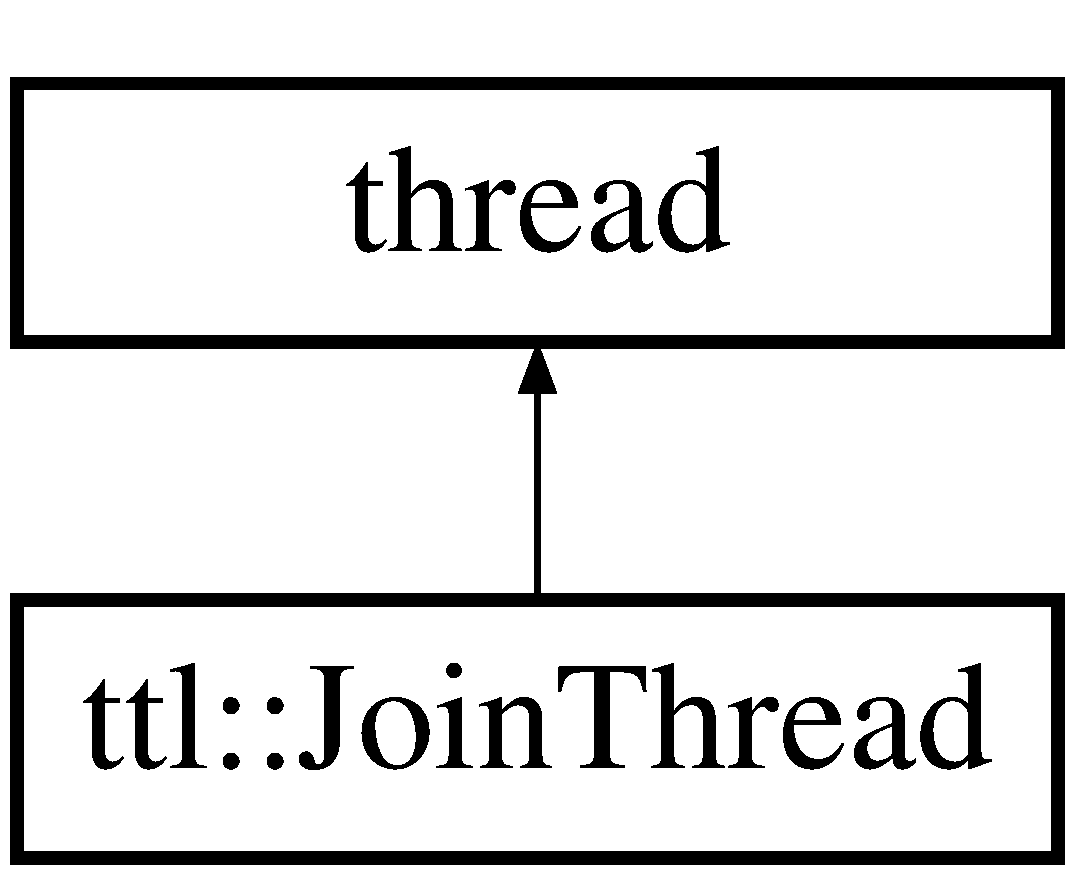
\includegraphics[height=2.000000cm]{classttl_1_1_join_thread}
\end{center}
\end{figure}
\subsection*{Public Member Functions}
\begin{DoxyCompactItemize}
\item 
\hyperlink{classttl_1_1_join_thread_a36602d0c8503ddf562a89b07c5ee7f34}{$\sim$\-Join\-Thread} ()
\begin{DoxyCompactList}\small\item\em Constructor delegator. \end{DoxyCompactList}\end{DoxyCompactItemize}


\subsection{Detailed Description}
Scoped thread that joins at scope exit. 

\subsection{Constructor \& Destructor Documentation}
\hypertarget{classttl_1_1_join_thread_a36602d0c8503ddf562a89b07c5ee7f34}{\index{ttl\-::\-Join\-Thread@{ttl\-::\-Join\-Thread}!$\sim$\-Join\-Thread@{$\sim$\-Join\-Thread}}
\index{$\sim$\-Join\-Thread@{$\sim$\-Join\-Thread}!ttl::JoinThread@{ttl\-::\-Join\-Thread}}
\subsubsection[{$\sim$\-Join\-Thread}]{\setlength{\rightskip}{0pt plus 5cm}ttl\-::\-Join\-Thread\-::$\sim$\-Join\-Thread (
\begin{DoxyParamCaption}
{}
\end{DoxyParamCaption}
)}}\label{classttl_1_1_join_thread_a36602d0c8503ddf562a89b07c5ee7f34}


Constructor delegator. 

\begin{DoxySeeAlso}{See Also}
std\-::thread\-::thread(...) Constructor delegator

std\-::thread\-::thread(...) Destructor
\end{DoxySeeAlso}
Joins the thread 

The documentation for this class was generated from the following file\-:\begin{DoxyCompactItemize}
\item 
include/\-Join\-Thread/Join\-Thread.\-hpp\end{DoxyCompactItemize}

\hypertarget{class_join_thread}{\section{Join\-Thread Class Reference}
\label{class_join_thread}\index{Join\-Thread@{Join\-Thread}}
}


{\ttfamily \#include $<$Join\-Thread.\-hpp$>$}



\subsection{Detailed Description}
This class works exactly like std\-::thread since it inherits therefrom and delegates all constructor arguments to std\-::thread\-::thread(...)


\begin{DoxyCode}
*  \textcolor{keywordtype}{int} &n = 0;
*  \hyperlink{class_join_thread}{JoinThread} thr
*  (
*      [](\textcolor{keywordtype}{int} &number)
*      \{
*          number++;
*          std::this\_thread::sleep\_for(std::chrono::seconds(3));
*      \},
*      std::ref(n)
*  );
*  
\end{DoxyCode}


Don't worry about detaching the thread, a check is performed during destruction to make sure the thread is joinable.

\begin{DoxySeeAlso}{See Also}
std\-::thread 
\end{DoxySeeAlso}


The documentation for this class was generated from the following file\-:\begin{DoxyCompactItemize}
\item 
include/\-Join\-Thread/Join\-Thread.\-hpp\end{DoxyCompactItemize}

\hypertarget{class_logger}{\section{Logger Class Reference}
\label{class_logger}\index{Logger@{Logger}}
}


{\ttfamily \#include $<$Logger.\-hpp$>$}



\subsection{Detailed Description}
This class will log to a file with an optional timestamp and other data. Changing the template argument turns the logger on and off, thus allowing the programmer to turn off the logger by changing a single argument, whilst leaving the logging code intact. This allows for easy debugging and information fetching.


\begin{DoxyCode}
*  \hyperlink{class_logger}{Logger<true>} log(\textcolor{stringliteral}{"messages.log"});
*  log << \textcolor{stringliteral}{"A message"};
*  
\end{DoxyCode}
 

The documentation for this class was generated from the following file\-:\begin{DoxyCompactItemize}
\item 
include/\-Logger/Logger.\-hpp\end{DoxyCompactItemize}

\hypertarget{classttl_1_1_logger}{\section{ttl\-:\-:Logger$<$ State $>$ Class Template Reference}
\label{classttl_1_1_logger}\index{ttl\-::\-Logger$<$ State $>$@{ttl\-::\-Logger$<$ State $>$}}
}


Simple logging utility.  




{\ttfamily \#include $<$Logger.\-hpp$>$}



\subsection{Detailed Description}
\subsubsection*{template$<$bool State$>$class ttl\-::\-Logger$<$ State $>$}

Simple logging utility. 

This class will log to a file with an optional timestamp and other data. Changing the template argument turns the logger on and off, thus allowing the programmer to turn off the logger by changing a single argument, whilst leaving the logging code intact. This allows for easy debugging and information fetching.


\begin{DoxyCode}
*  Logger<true> log(\textcolor{stringliteral}{"messages.log"});
*  log << \textcolor{stringliteral}{"A message"};
*  
\end{DoxyCode}
 

The documentation for this class was generated from the following file\-:\begin{DoxyCompactItemize}
\item 
include/\-Logger/Logger.\-hpp\end{DoxyCompactItemize}

\hypertarget{classttl_1_1_logger_3_01false_01_4}{\section{ttl\-:\-:Logger$<$ false $>$ Class Template Reference}
\label{classttl_1_1_logger_3_01false_01_4}\index{ttl\-::\-Logger$<$ false $>$@{ttl\-::\-Logger$<$ false $>$}}
}


Simple logging utility -\/ False part.  




{\ttfamily \#include $<$Logger.\-hpp$>$}

\subsection*{Public Member Functions}
\begin{DoxyCompactItemize}
\item 
\hypertarget{classttl_1_1_logger_3_01false_01_4_a51ebd004cd57d3f20c074292956909da}{{\bfseries Logger} (const char $\ast$filename=\char`\"{}log.\-log\char`\"{}, bool to\-\_\-clog=true, std\-::ios\-::openmode std\-\_\-ios\-\_\-flags=std\-::ios\-::out$|$std\-::ios\-::app)}\label{classttl_1_1_logger_3_01false_01_4_a51ebd004cd57d3f20c074292956909da}

\item 
\hypertarget{classttl_1_1_logger_3_01false_01_4_a56b1a3fa243bee87024d96f0f31bde5f}{{\bfseries Logger} (std\-::string \&filename, bool to\-\_\-clog=true, std\-::ios\-::openmode std\-\_\-ios\-\_\-flags=std\-::ios\-::out$|$std\-::ios\-::app)}\label{classttl_1_1_logger_3_01false_01_4_a56b1a3fa243bee87024d96f0f31bde5f}

\item 
\hypertarget{classttl_1_1_logger_3_01false_01_4_a1f17d7e08362e7f9a1ab661c64468362}{{\footnotesize template$<$typename T $>$ }\\\hyperlink{classttl_1_1_logger}{Logger} \& {\bfseries operator$<$$<$} (T \&\&rhs)}\label{classttl_1_1_logger_3_01false_01_4_a1f17d7e08362e7f9a1ab661c64468362}

\end{DoxyCompactItemize}


\subsection{Detailed Description}
\subsubsection*{template$<$$>$class ttl\-::\-Logger$<$ false $>$}

Simple logging utility -\/ False part. 

The false part is a specialized template that disables all logger functionality. The compiler is likely to optimize away the empty function calls resulting in an object that literally does nothing in running code. There is also no data usage at all.

\begin{DoxySeeAlso}{See Also}
\hyperlink{classttl_1_1_logger_3_01true_01_4}{Logger$<$true$>$} 
\end{DoxySeeAlso}


The documentation for this class was generated from the following file\-:\begin{DoxyCompactItemize}
\item 
include/\-Logger/Logger.\-hpp\end{DoxyCompactItemize}

\hypertarget{classttl_1_1_logger_3_01true_01_4}{\section{ttl\-:\-:Logger$<$ true $>$ Class Template Reference}
\label{classttl_1_1_logger_3_01true_01_4}\index{ttl\-::\-Logger$<$ true $>$@{ttl\-::\-Logger$<$ true $>$}}
}


Simple logging utility -\/ True part.  




{\ttfamily \#include $<$Logger.\-hpp$>$}

\subsection*{Public Member Functions}
\begin{DoxyCompactItemize}
\item 
\hyperlink{classttl_1_1_logger_3_01true_01_4_a6068268c9c9383f89c7ff3411588c04d}{Logger} (const char $\ast$filename=\char`\"{}log.\-log\char`\"{}, bool to\-\_\-clog=true, std\-::ios\-::openmode std\-\_\-ios\-\_\-flags=std\-::ios\-::out$|$std\-::ios\-::app)
\begin{DoxyCompactList}\small\item\em Constructor. \end{DoxyCompactList}\item 
\hyperlink{classttl_1_1_logger_3_01true_01_4_afa7eedcdc4d0ab642d35de8fa7038929}{Logger} (std\-::string \&filename, bool to\-\_\-clog=true, std\-::ios\-::openmode std\-\_\-ios\-\_\-flags=std\-::ios\-::out$|$std\-::ios\-::app)
\begin{DoxyCompactList}\small\item\em Constructor. \end{DoxyCompactList}\item 
\hypertarget{classttl_1_1_logger_3_01true_01_4_a353d04b6a0a678a38c3c9ff194cd8486}{\hyperlink{classttl_1_1_logger_3_01true_01_4_a353d04b6a0a678a38c3c9ff194cd8486}{$\sim$\-Logger} ()}\label{classttl_1_1_logger_3_01true_01_4_a353d04b6a0a678a38c3c9ff194cd8486}

\begin{DoxyCompactList}\small\item\em Destructor. \end{DoxyCompactList}\item 
{\footnotesize template$<$typename T $>$ }\\\hyperlink{classttl_1_1_logger}{Logger} \& \hyperlink{classttl_1_1_logger_3_01true_01_4_ab08287107b52a13d8007397d206bee9b}{operator$<$$<$} (T \&\&rhs)
\begin{DoxyCompactList}\small\item\em Operator$<$$<$. \end{DoxyCompactList}\item 
\hypertarget{classttl_1_1_logger_3_01true_01_4_a8b967c1325694484d50130f0752aac9a}{\hyperlink{classttl_1_1_logger}{Logger} \& {\bfseries operator$<$$<$} (\hyperlink{structttl_1_1m___timestamp}{m\-\_\-\-Timestamp})}\label{classttl_1_1_logger_3_01true_01_4_a8b967c1325694484d50130f0752aac9a}

\end{DoxyCompactItemize}


\subsection{Detailed Description}
\subsubsection*{template$<$$>$class ttl\-::\-Logger$<$ true $>$}

Simple logging utility -\/ True part. 

The true specialized template for \hyperlink{classttl_1_1_logger}{Logger} is the part that actually logs when requested to do so. It keeps open an fstream to the file it is supposed to write to.

\begin{DoxySeeAlso}{See Also}
\hyperlink{classttl_1_1_logger_3_01false_01_4}{Logger$<$false$>$} 
\end{DoxySeeAlso}


\subsection{Constructor \& Destructor Documentation}
\hypertarget{classttl_1_1_logger_3_01true_01_4_a6068268c9c9383f89c7ff3411588c04d}{\index{ttl\-::\-Logger$<$ true $>$@{ttl\-::\-Logger$<$ true $>$}!Logger@{Logger}}
\index{Logger@{Logger}!ttl::Logger< true >@{ttl\-::\-Logger$<$ true $>$}}
\subsubsection[{Logger}]{\setlength{\rightskip}{0pt plus 5cm}{\bf ttl\-::\-Logger}$<$ true $>$\-::{\bf Logger} (
\begin{DoxyParamCaption}
\item[{const char $\ast$}]{filename = {\ttfamily \char`\"{}log.log\char`\"{}}, }
\item[{bool}]{to\-\_\-clog = {\ttfamily true}, }
\item[{std\-::ios\-::openmode}]{std\-\_\-ios\-\_\-flags = {\ttfamily std\-:\-:ios\-:\-:out$|$std\-:\-:ios\-:\-:app}}
\end{DoxyParamCaption}
)\hspace{0.3cm}{\ttfamily [explicit]}}}\label{classttl_1_1_logger_3_01true_01_4_a6068268c9c9383f89c7ff3411588c04d}


Constructor. 


\begin{DoxyParams}{Parameters}
{\em filename} & The file name and location \\
\hline
{\em to\-\_\-clog} & Whether to output to std\-::clog ostream or not \\
\hline
{\em std\-\_\-ios\-\_\-flags} & The mode to open the file in\\
\hline
\end{DoxyParams}
\begin{DoxySeeAlso}{See Also}
std\-::ios\-::openmode 
\end{DoxySeeAlso}
\hypertarget{classttl_1_1_logger_3_01true_01_4_afa7eedcdc4d0ab642d35de8fa7038929}{\index{ttl\-::\-Logger$<$ true $>$@{ttl\-::\-Logger$<$ true $>$}!Logger@{Logger}}
\index{Logger@{Logger}!ttl::Logger< true >@{ttl\-::\-Logger$<$ true $>$}}
\subsubsection[{Logger}]{\setlength{\rightskip}{0pt plus 5cm}{\bf ttl\-::\-Logger}$<$ true $>$\-::{\bf Logger} (
\begin{DoxyParamCaption}
\item[{std\-::string \&}]{filename, }
\item[{bool}]{to\-\_\-clog = {\ttfamily true}, }
\item[{std\-::ios\-::openmode}]{std\-\_\-ios\-\_\-flags = {\ttfamily std\-:\-:ios\-:\-:out$|$std\-:\-:ios\-:\-:app}}
\end{DoxyParamCaption}
)\hspace{0.3cm}{\ttfamily [explicit]}}}\label{classttl_1_1_logger_3_01true_01_4_afa7eedcdc4d0ab642d35de8fa7038929}


Constructor. 


\begin{DoxyParams}{Parameters}
{\em filename} & The file name and location \\
\hline
{\em to\-\_\-clog} & Whether to output to std\-::clog ostream or not \\
\hline
{\em std\-\_\-ios\-\_\-flags} & The mode to open the file in\\
\hline
\end{DoxyParams}
\begin{DoxySeeAlso}{See Also}
std\-::ios\-::openmode 
\end{DoxySeeAlso}


\subsection{Member Function Documentation}
\hypertarget{classttl_1_1_logger_3_01true_01_4_ab08287107b52a13d8007397d206bee9b}{\index{ttl\-::\-Logger$<$ true $>$@{ttl\-::\-Logger$<$ true $>$}!operator$<$$<$@{operator$<$$<$}}
\index{operator$<$$<$@{operator$<$$<$}!ttl::Logger< true >@{ttl\-::\-Logger$<$ true $>$}}
\subsubsection[{operator$<$$<$}]{\setlength{\rightskip}{0pt plus 5cm}template$<$typename T $>$ {\bf Logger}\& {\bf ttl\-::\-Logger}$<$ true $>$\-::operator$<$$<$ (
\begin{DoxyParamCaption}
\item[{T \&\&}]{rhs}
\end{DoxyParamCaption}
)\hspace{0.3cm}{\ttfamily [inline]}}}\label{classttl_1_1_logger_3_01true_01_4_ab08287107b52a13d8007397d206bee9b}


Operator$<$$<$. 


\begin{DoxyParams}{Parameters}
{\em rhs} & The argument to add to the log\\
\hline
\end{DoxyParams}
\begin{DoxySeeAlso}{See Also}
std\-::ostream\-::operator$<$$<$ 
\end{DoxySeeAlso}


The documentation for this class was generated from the following file\-:\begin{DoxyCompactItemize}
\item 
include/\-Logger/Logger.\-hpp\end{DoxyCompactItemize}

\hypertarget{structttl_1_1m___timestamp}{\section{ttl\-:\-:m\-\_\-\-Timestamp Struct Reference}
\label{structttl_1_1m___timestamp}\index{ttl\-::m\-\_\-\-Timestamp@{ttl\-::m\-\_\-\-Timestamp}}
}


Dummy variable used in \hyperlink{classttl_1_1_logger}{Logger} for overloads.  




{\ttfamily \#include $<$Timestamp.\-hpp$>$}



\subsection{Detailed Description}
Dummy variable used in \hyperlink{classttl_1_1_logger}{Logger} for overloads. 

The documentation for this struct was generated from the following file\-:\begin{DoxyCompactItemize}
\item 
include/\-Timestamp/Timestamp.\-hpp\end{DoxyCompactItemize}

\hypertarget{classttl_1_1_mixin}{\section{ttl\-:\-:Mixin$<$ C\-L\-A\-S\-S\-E\-S $>$ Class Template Reference}
\label{classttl_1_1_mixin}\index{ttl\-::\-Mixin$<$ C\-L\-A\-S\-S\-E\-S $>$@{ttl\-::\-Mixin$<$ C\-L\-A\-S\-S\-E\-S $>$}}
}


A class for mixing classes with eachother.  




{\ttfamily \#include $<$Mixin.\-hpp$>$}

Inheritance diagram for ttl\-:\-:Mixin$<$ C\-L\-A\-S\-S\-E\-S $>$\-:\begin{figure}[H]
\begin{center}
\leavevmode
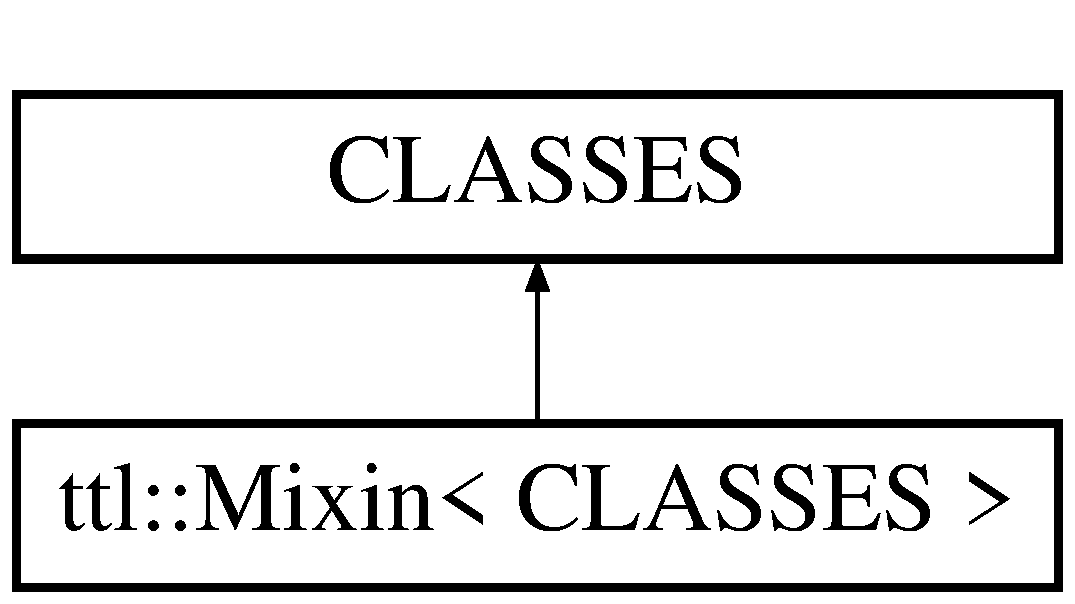
\includegraphics[height=2.000000cm]{classttl_1_1_mixin}
\end{center}
\end{figure}
\subsection*{Public Member Functions}
\begin{DoxyCompactItemize}
\item 
\hyperlink{classttl_1_1_mixin_a7b9697018f0edc09abc9bc3d6a4e2010}{Mixin} ()
\begin{DoxyCompactList}\small\item\em Constructor. \end{DoxyCompactList}\end{DoxyCompactItemize}


\subsection{Detailed Description}
\subsubsection*{template$<$typename... C\-L\-A\-S\-S\-E\-S$>$class ttl\-::\-Mixin$<$ C\-L\-A\-S\-S\-E\-S $>$}

A class for mixing classes with eachother. 

\subsection{Constructor \& Destructor Documentation}
\hypertarget{classttl_1_1_mixin_a7b9697018f0edc09abc9bc3d6a4e2010}{\index{ttl\-::\-Mixin@{ttl\-::\-Mixin}!Mixin@{Mixin}}
\index{Mixin@{Mixin}!ttl::Mixin@{ttl\-::\-Mixin}}
\subsubsection[{Mixin}]{\setlength{\rightskip}{0pt plus 5cm}template$<$typename... C\-L\-A\-S\-S\-E\-S$>$ {\bf ttl\-::\-Mixin}$<$ C\-L\-A\-S\-S\-E\-S $>$\-::{\bf Mixin} (
\begin{DoxyParamCaption}
{}
\end{DoxyParamCaption}
)\hspace{0.3cm}{\ttfamily [inline]}, {\ttfamily [explicit]}}}\label{classttl_1_1_mixin_a7b9697018f0edc09abc9bc3d6a4e2010}


Constructor. 

Using template arguments, constructs the classes 

The documentation for this class was generated from the following file\-:\begin{DoxyCompactItemize}
\item 
include/\-Mixin/Mixin.\-hpp\end{DoxyCompactItemize}

\hypertarget{classttl_1_1_runnable}{\section{ttl\-:\-:Runnable Class Reference}
\label{classttl_1_1_runnable}\index{ttl\-::\-Runnable@{ttl\-::\-Runnable}}
}


Class for managing cycles of runnable objects.  




{\ttfamily \#include $<$Runnable.\-hpp$>$}

\subsection*{Public Member Functions}
\begin{DoxyCompactItemize}
\item 
\hypertarget{classttl_1_1_runnable_af6956d428e33c97a44fe01e707f20c49}{virtual \hyperlink{classttl_1_1_runnable}{Runnable} $\ast$ {\bfseries run} ()=0}\label{classttl_1_1_runnable_af6956d428e33c97a44fe01e707f20c49}

\end{DoxyCompactItemize}
\subsection*{Static Public Member Functions}
\begin{DoxyCompactItemize}
\item 
\hypertarget{classttl_1_1_runnable_aa959aaca8db913584fba289ee9119344}{static void \hyperlink{classttl_1_1_runnable_aa959aaca8db913584fba289ee9119344}{cycle} (std\-::unique\-\_\-ptr$<$ \hyperlink{classttl_1_1_runnable}{Runnable} $>$ runnable)}\label{classttl_1_1_runnable_aa959aaca8db913584fba289ee9119344}

\begin{DoxyCompactList}\small\item\em Handles exceptions and logs times. \end{DoxyCompactList}\end{DoxyCompactItemize}


\subsection{Detailed Description}
Class for managing cycles of runnable objects. 

Inheriting from this class and overriding its run function will allow you to send such class into \hyperlink{classttl_1_1_runnable_aa959aaca8db913584fba289ee9119344}{ttl\-::\-Runnable\-::cycle} 

The documentation for this class was generated from the following file\-:\begin{DoxyCompactItemize}
\item 
include/\-Runnable/Runnable.\-hpp\end{DoxyCompactItemize}

\hypertarget{classttl_1_1_synched}{\section{ttl\-:\-:Synched$<$ T $>$ Class Template Reference}
\label{classttl_1_1_synched}\index{ttl\-::\-Synched$<$ T $>$@{ttl\-::\-Synched$<$ T $>$}}
}


Encapsulator that makes objects thread safe.  




{\ttfamily \#include $<$Synched.\-hpp$>$}

\subsection*{Public Member Functions}
\begin{DoxyCompactItemize}
\item 
\hyperlink{classttl_1_1_synched_afb711c74345c0fe671313e6df9a38fb1}{Synched} ()=default
\begin{DoxyCompactList}\small\item\em Default ctor. \end{DoxyCompactList}\item 
{\footnotesize template$<$typename... Args$>$ }\\\hyperlink{classttl_1_1_synched_a3682a5a65a6871126e0fefbd6b335482}{Synched} (Args...\-args)
\begin{DoxyCompactList}\small\item\em Argument ctor. \end{DoxyCompactList}\item 
\hyperlink{classttl_1_1_synched_aa0699d5888f20a1df6e53303700f40a0}{Synched} (const T \&in)
\begin{DoxyCompactList}\small\item\em Copy ctor. \end{DoxyCompactList}\item 
\hyperlink{classttl_1_1_synched_af2abfc5aa8f9246420947816d06ba26f}{Synched} (T \&\&in)
\begin{DoxyCompactList}\small\item\em Move ctor. \end{DoxyCompactList}\item 
\hyperlink{classttl_1_1_synched_a256002a4a8d0f0b4fe75c7a8b2902698}{Synched} (const \hyperlink{classttl_1_1_synched}{Synched} \&copy)
\begin{DoxyCompactList}\small\item\em Copy ctor. \end{DoxyCompactList}\item 
\hyperlink{classttl_1_1_synched_a647dfd353e18d2986cf210db056af49c}{Synched} (\hyperlink{classttl_1_1_synched}{Synched} \&\&copy)
\begin{DoxyCompactList}\small\item\em Move ctor. \end{DoxyCompactList}\item 
\hyperlink{classttl_1_1_synched}{Synched} \& \hyperlink{classttl_1_1_synched_ae7dbfca4dc7944c22b408bf191c90786}{operator=} (const \hyperlink{classttl_1_1_synched}{Synched} \&copy)
\begin{DoxyCompactList}\small\item\em Copy assignment. \end{DoxyCompactList}\item 
\hyperlink{classttl_1_1_synched}{Synched} \& \hyperlink{classttl_1_1_synched_a21494a85d6afe4c47cc640acee86c6d4}{operator=} (\hyperlink{classttl_1_1_synched}{Synched} \&\&copy)
\begin{DoxyCompactList}\small\item\em Move assignment. \end{DoxyCompactList}\item 
\hyperlink{classttl_1_1_synched_ac8f8ec455e4fcfdabb0dc75d516e79ec}{$\sim$\-Synched} ()=default
\begin{DoxyCompactList}\small\item\em Destructor. \end{DoxyCompactList}\item 
\hyperlink{classttl_1_1_synched_writer}{Synched\-Writer}$<$ T $>$ \hyperlink{classttl_1_1_synched_a913a8d279fad4d94649dee596278a3dd}{get\-Write\-Access} ()
\begin{DoxyCompactList}\small\item\em returns a \hyperlink{classttl_1_1_synched_writer}{Synched\-Writer} \end{DoxyCompactList}\item 
const \hyperlink{classttl_1_1_synched_reader}{Synched\-Reader}$<$ T $>$ \hyperlink{classttl_1_1_synched_a88e58e2776f408481de37ae8ce89c6b1}{get\-Read\-Access} () const 
\begin{DoxyCompactList}\small\item\em returns a \hyperlink{classttl_1_1_synched_reader}{Synched\-Reader} \end{DoxyCompactList}\item 
std\-::size\-\_\-t \hyperlink{classttl_1_1_synched_aa6694d8a6541730ea80a8844c4d267e3}{get\-Reader\-Count} () const 
\begin{DoxyCompactList}\small\item\em The count of readers. \end{DoxyCompactList}\end{DoxyCompactItemize}


\subsection{Detailed Description}
\subsubsection*{template$<$typename T$>$class ttl\-::\-Synched$<$ T $>$}

Encapsulator that makes objects thread safe. 

Allows multiple reads, but only single writes. This implementation is A\-L\-W\-A\-Y\-S thread-\/safe, unless multiple readers edit mutable variables simultaneously. This depends on the class at hand. If your class has mutable fields, then make sure to make all const functions take note of that (and protect it). Another option is to make the mutable a Synched$<$$>$ object. 

\subsection{Constructor \& Destructor Documentation}
\hypertarget{classttl_1_1_synched_afb711c74345c0fe671313e6df9a38fb1}{\index{ttl\-::\-Synched@{ttl\-::\-Synched}!Synched@{Synched}}
\index{Synched@{Synched}!ttl::Synched@{ttl\-::\-Synched}}
\subsubsection[{Synched}]{\setlength{\rightskip}{0pt plus 5cm}template$<$typename T$>$ {\bf ttl\-::\-Synched}$<$ T $>$\-::{\bf Synched} (
\begin{DoxyParamCaption}
{}
\end{DoxyParamCaption}
)\hspace{0.3cm}{\ttfamily [default]}}}\label{classttl_1_1_synched_afb711c74345c0fe671313e6df9a38fb1}


Default ctor. 

Will invoke the data's standard ctor. Can be garbage data. \hypertarget{classttl_1_1_synched_a3682a5a65a6871126e0fefbd6b335482}{\index{ttl\-::\-Synched@{ttl\-::\-Synched}!Synched@{Synched}}
\index{Synched@{Synched}!ttl::Synched@{ttl\-::\-Synched}}
\subsubsection[{Synched}]{\setlength{\rightskip}{0pt plus 5cm}template$<$typename T$>$ template$<$typename... Args$>$ {\bf ttl\-::\-Synched}$<$ T $>$\-::{\bf Synched} (
\begin{DoxyParamCaption}
\item[{Args...}]{args}
\end{DoxyParamCaption}
)\hspace{0.3cm}{\ttfamily [inline]}}}\label{classttl_1_1_synched_a3682a5a65a6871126e0fefbd6b335482}


Argument ctor. 


\begin{DoxyParams}{Parameters}
{\em args} & Forwards the arguments to the constructor of the data specified in the template. \\
\hline
\end{DoxyParams}
\hypertarget{classttl_1_1_synched_aa0699d5888f20a1df6e53303700f40a0}{\index{ttl\-::\-Synched@{ttl\-::\-Synched}!Synched@{Synched}}
\index{Synched@{Synched}!ttl::Synched@{ttl\-::\-Synched}}
\subsubsection[{Synched}]{\setlength{\rightskip}{0pt plus 5cm}template$<$typename T$>$ {\bf ttl\-::\-Synched}$<$ T $>$\-::{\bf Synched} (
\begin{DoxyParamCaption}
\item[{const T \&}]{in}
\end{DoxyParamCaption}
)\hspace{0.3cm}{\ttfamily [inline]}}}\label{classttl_1_1_synched_aa0699d5888f20a1df6e53303700f40a0}


Copy ctor. 

Copies the data an external source \hypertarget{classttl_1_1_synched_af2abfc5aa8f9246420947816d06ba26f}{\index{ttl\-::\-Synched@{ttl\-::\-Synched}!Synched@{Synched}}
\index{Synched@{Synched}!ttl::Synched@{ttl\-::\-Synched}}
\subsubsection[{Synched}]{\setlength{\rightskip}{0pt plus 5cm}template$<$typename T$>$ {\bf ttl\-::\-Synched}$<$ T $>$\-::{\bf Synched} (
\begin{DoxyParamCaption}
\item[{T \&\&}]{in}
\end{DoxyParamCaption}
)\hspace{0.3cm}{\ttfamily [inline]}}}\label{classttl_1_1_synched_af2abfc5aa8f9246420947816d06ba26f}


Move ctor. 

Copies the data from an r-\/value reference. \hypertarget{classttl_1_1_synched_a256002a4a8d0f0b4fe75c7a8b2902698}{\index{ttl\-::\-Synched@{ttl\-::\-Synched}!Synched@{Synched}}
\index{Synched@{Synched}!ttl::Synched@{ttl\-::\-Synched}}
\subsubsection[{Synched}]{\setlength{\rightskip}{0pt plus 5cm}template$<$typename T$>$ {\bf ttl\-::\-Synched}$<$ T $>$\-::{\bf Synched} (
\begin{DoxyParamCaption}
\item[{const {\bf Synched}$<$ T $>$ \&}]{copy}
\end{DoxyParamCaption}
)\hspace{0.3cm}{\ttfamily [inline]}}}\label{classttl_1_1_synched_a256002a4a8d0f0b4fe75c7a8b2902698}


Copy ctor. 

Copies the data contained in another \hyperlink{classttl_1_1_synched}{Synched} object \hypertarget{classttl_1_1_synched_a647dfd353e18d2986cf210db056af49c}{\index{ttl\-::\-Synched@{ttl\-::\-Synched}!Synched@{Synched}}
\index{Synched@{Synched}!ttl::Synched@{ttl\-::\-Synched}}
\subsubsection[{Synched}]{\setlength{\rightskip}{0pt plus 5cm}template$<$typename T$>$ {\bf ttl\-::\-Synched}$<$ T $>$\-::{\bf Synched} (
\begin{DoxyParamCaption}
\item[{{\bf Synched}$<$ T $>$ \&\&}]{copy}
\end{DoxyParamCaption}
)\hspace{0.3cm}{\ttfamily [inline]}}}\label{classttl_1_1_synched_a647dfd353e18d2986cf210db056af49c}


Move ctor. 

Moves the data contained in another \hyperlink{classttl_1_1_synched}{Synched} object \hypertarget{classttl_1_1_synched_ac8f8ec455e4fcfdabb0dc75d516e79ec}{\index{ttl\-::\-Synched@{ttl\-::\-Synched}!$\sim$\-Synched@{$\sim$\-Synched}}
\index{$\sim$\-Synched@{$\sim$\-Synched}!ttl::Synched@{ttl\-::\-Synched}}
\subsubsection[{$\sim$\-Synched}]{\setlength{\rightskip}{0pt plus 5cm}template$<$typename T$>$ {\bf ttl\-::\-Synched}$<$ T $>$\-::$\sim${\bf Synched} (
\begin{DoxyParamCaption}
{}
\end{DoxyParamCaption}
)\hspace{0.3cm}{\ttfamily [default]}}}\label{classttl_1_1_synched_ac8f8ec455e4fcfdabb0dc75d516e79ec}


Destructor. 

Everything is R\-A\-I\-I, no need to do anything 

\subsection{Member Function Documentation}
\hypertarget{classttl_1_1_synched_a88e58e2776f408481de37ae8ce89c6b1}{\index{ttl\-::\-Synched@{ttl\-::\-Synched}!get\-Read\-Access@{get\-Read\-Access}}
\index{get\-Read\-Access@{get\-Read\-Access}!ttl::Synched@{ttl\-::\-Synched}}
\subsubsection[{get\-Read\-Access}]{\setlength{\rightskip}{0pt plus 5cm}template$<$typename T$>$ const {\bf Synched\-Reader}$<$T$>$ {\bf ttl\-::\-Synched}$<$ T $>$\-::get\-Read\-Access (
\begin{DoxyParamCaption}
{}
\end{DoxyParamCaption}
) const\hspace{0.3cm}{\ttfamily [inline]}}}\label{classttl_1_1_synched_a88e58e2776f408481de37ae8ce89c6b1}


returns a \hyperlink{classttl_1_1_synched_reader}{Synched\-Reader} 

The \hyperlink{classttl_1_1_synched_reader}{Synched\-Reader} will block all Synched\-Writers until all Synched\-Readers have been destroyed.

\begin{DoxyReturn}{Returns}
a \hyperlink{classttl_1_1_synched_reader}{Synched\-Reader} object 
\end{DoxyReturn}
\hypertarget{classttl_1_1_synched_aa6694d8a6541730ea80a8844c4d267e3}{\index{ttl\-::\-Synched@{ttl\-::\-Synched}!get\-Reader\-Count@{get\-Reader\-Count}}
\index{get\-Reader\-Count@{get\-Reader\-Count}!ttl::Synched@{ttl\-::\-Synched}}
\subsubsection[{get\-Reader\-Count}]{\setlength{\rightskip}{0pt plus 5cm}template$<$typename T$>$ std\-::size\-\_\-t {\bf ttl\-::\-Synched}$<$ T $>$\-::get\-Reader\-Count (
\begin{DoxyParamCaption}
{}
\end{DoxyParamCaption}
) const\hspace{0.3cm}{\ttfamily [inline]}}}\label{classttl_1_1_synched_aa6694d8a6541730ea80a8844c4d267e3}


The count of readers. 

\begin{DoxyReturn}{Returns}
the amount of readers currently reading the data. 
\end{DoxyReturn}
\hypertarget{classttl_1_1_synched_a913a8d279fad4d94649dee596278a3dd}{\index{ttl\-::\-Synched@{ttl\-::\-Synched}!get\-Write\-Access@{get\-Write\-Access}}
\index{get\-Write\-Access@{get\-Write\-Access}!ttl::Synched@{ttl\-::\-Synched}}
\subsubsection[{get\-Write\-Access}]{\setlength{\rightskip}{0pt plus 5cm}template$<$typename T$>$ {\bf Synched\-Writer}$<$T$>$ {\bf ttl\-::\-Synched}$<$ T $>$\-::get\-Write\-Access (
\begin{DoxyParamCaption}
{}
\end{DoxyParamCaption}
)\hspace{0.3cm}{\ttfamily [inline]}}}\label{classttl_1_1_synched_a913a8d279fad4d94649dee596278a3dd}


returns a \hyperlink{classttl_1_1_synched_writer}{Synched\-Writer} 

Waits for all Synched\-Readers to be destroyed. The \hyperlink{classttl_1_1_synched_writer}{Synched\-Writer} will block all other writers and readers until its destructor has been called.

\begin{DoxyReturn}{Returns}
a \hyperlink{classttl_1_1_synched_writer}{Synched\-Writer} object 
\end{DoxyReturn}
\hypertarget{classttl_1_1_synched_ae7dbfca4dc7944c22b408bf191c90786}{\index{ttl\-::\-Synched@{ttl\-::\-Synched}!operator=@{operator=}}
\index{operator=@{operator=}!ttl::Synched@{ttl\-::\-Synched}}
\subsubsection[{operator=}]{\setlength{\rightskip}{0pt plus 5cm}template$<$typename T$>$ {\bf Synched}\& {\bf ttl\-::\-Synched}$<$ T $>$\-::operator= (
\begin{DoxyParamCaption}
\item[{const {\bf Synched}$<$ T $>$ \&}]{copy}
\end{DoxyParamCaption}
)\hspace{0.3cm}{\ttfamily [inline]}}}\label{classttl_1_1_synched_ae7dbfca4dc7944c22b408bf191c90786}


Copy assignment. 

Copies the data contained in another \hyperlink{classttl_1_1_synched}{Synched} object

\begin{DoxyReturn}{Returns}
A reference to itself 
\end{DoxyReturn}
\hypertarget{classttl_1_1_synched_a21494a85d6afe4c47cc640acee86c6d4}{\index{ttl\-::\-Synched@{ttl\-::\-Synched}!operator=@{operator=}}
\index{operator=@{operator=}!ttl::Synched@{ttl\-::\-Synched}}
\subsubsection[{operator=}]{\setlength{\rightskip}{0pt plus 5cm}template$<$typename T$>$ {\bf Synched}\& {\bf ttl\-::\-Synched}$<$ T $>$\-::operator= (
\begin{DoxyParamCaption}
\item[{{\bf Synched}$<$ T $>$ \&\&}]{copy}
\end{DoxyParamCaption}
)\hspace{0.3cm}{\ttfamily [inline]}}}\label{classttl_1_1_synched_a21494a85d6afe4c47cc640acee86c6d4}


Move assignment. 

Copies the data contained in another \hyperlink{classttl_1_1_synched}{Synched} object

\begin{DoxyReturn}{Returns}
A reference to itself 
\end{DoxyReturn}


The documentation for this class was generated from the following file\-:\begin{DoxyCompactItemize}
\item 
include/\-Synched/Synched.\-hpp\end{DoxyCompactItemize}

\hypertarget{class_synched}{\section{Synched Class Reference}
\label{class_synched}\index{Synched@{Synched}}
}


{\ttfamily \#include $<$Synched.\-hpp$>$}



\subsection{Detailed Description}
Using \hyperlink{class_synched}{Synched} will allow for multiple readers to read, whilst only a single writer can write at a time. The protective method is the same as the one employed by std\-::weak\-\_\-ptr. This method uses a temporary object.


\begin{DoxyCode}
*  \hyperlink{classttl_1_1_synched}{ttl::Synched<int>} xxx(32);
* 
*  \textcolor{comment}{// From thread 1:}
*  \textcolor{keyword}{auto} x = xxx.getReadAccess(); \textcolor{comment}{// Reader object, multiple can exist simultaneously.}
*  std::cout << *x << std::endl;
* 
*  \textcolor{comment}{// From thread 2:}
*  \textcolor{keyword}{auto} x = xxx.getWriteAccess(); \textcolor{comment}{// Writer object, no more than 1 can exist simultaneously.}
*  (*x)++;
* 
*  
\end{DoxyCode}
 

The documentation for this class was generated from the following file\-:\begin{DoxyCompactItemize}
\item 
include/\-Synched/Synched.\-hpp\end{DoxyCompactItemize}

\hypertarget{structttl_1_1_synched_data}{\section{ttl\-:\-:Synched\-Data Struct Reference}
\label{structttl_1_1_synched_data}\index{ttl\-::\-Synched\-Data@{ttl\-::\-Synched\-Data}}
}


Wrapper of \hyperlink{classttl_1_1_synched}{Synched}'s internal data.  




{\ttfamily \#include $<$Synched\-Data.\-hpp$>$}

\subsection*{Public Attributes}
\begin{DoxyCompactItemize}
\item 
\hypertarget{structttl_1_1_synched_data_a4249f85d2eb682541bbbe5daa7f3c57d}{std\-::mutex {\bfseries entry\-\_\-mutex}}\label{structttl_1_1_synched_data_a4249f85d2eb682541bbbe5daa7f3c57d}

\item 
\hypertarget{structttl_1_1_synched_data_a1e643d3a430790684d17070b85e852c1}{\hyperlink{classttl_1_1_flare}{ttl\-::\-Flare} {\bfseries writer\-\_\-activation}}\label{structttl_1_1_synched_data_a1e643d3a430790684d17070b85e852c1}

\item 
\hypertarget{structttl_1_1_synched_data_a3192f4eedc52ac010cda73e6b072414a}{std\-::atomic$<$ std\-::size\-\_\-t $>$ {\bfseries readers}}\label{structttl_1_1_synched_data_a3192f4eedc52ac010cda73e6b072414a}

\end{DoxyCompactItemize}


\subsection{Detailed Description}
Wrapper of \hyperlink{classttl_1_1_synched}{Synched}'s internal data. 

The documentation for this struct was generated from the following file\-:\begin{DoxyCompactItemize}
\item 
include/\-Synched/Synched\-Data.\-hpp\end{DoxyCompactItemize}

\hypertarget{classttl_1_1_synched_reader}{\section{ttl\-:\-:Synched\-Reader$<$ T $>$ Class Template Reference}
\label{classttl_1_1_synched_reader}\index{ttl\-::\-Synched\-Reader$<$ T $>$@{ttl\-::\-Synched\-Reader$<$ T $>$}}
}


The reader object.  




{\ttfamily \#include $<$Synched\-Reader.\-hpp$>$}

\subsection*{Public Member Functions}
\begin{DoxyCompactItemize}
\item 
\hyperlink{classttl_1_1_synched_reader_a372c3edad0bb203d4020db4cf37dfd5a}{Synched\-Reader} (\hyperlink{structttl_1_1_synched_data}{Synched\-Data} \&synch, const T \&data)
\begin{DoxyCompactList}\small\item\em Constructor. \end{DoxyCompactList}\item 
\hyperlink{classttl_1_1_synched_reader_a1074be7ecda55d0ed6b729781773d160}{$\sim$\-Synched\-Reader} ()
\begin{DoxyCompactList}\small\item\em Destructor. \end{DoxyCompactList}\item 
const T $\ast$ \hyperlink{classttl_1_1_synched_reader_a49fe60c81e1a0311eb9a5a1ae2c778e8}{operator-\/$>$} () const 
\begin{DoxyCompactList}\small\item\em Data extraction. \end{DoxyCompactList}\item 
const T \& \hyperlink{classttl_1_1_synched_reader_a1a36614df1ac988950c548af532047bb}{operator$\ast$} () const 
\begin{DoxyCompactList}\small\item\em Data extraction. \end{DoxyCompactList}\item 
std\-::size\-\_\-t \hyperlink{classttl_1_1_synched_reader_a5bf67d186e49a9dc45f93379b6cf474c}{get\-Reader\-Count} () const 
\begin{DoxyCompactList}\small\item\em The count of readers. \end{DoxyCompactList}\end{DoxyCompactItemize}


\subsection{Detailed Description}
\subsubsection*{template$<$typename T$>$class ttl\-::\-Synched\-Reader$<$ T $>$}

The reader object. 

\subsection{Constructor \& Destructor Documentation}
\hypertarget{classttl_1_1_synched_reader_a372c3edad0bb203d4020db4cf37dfd5a}{\index{ttl\-::\-Synched\-Reader@{ttl\-::\-Synched\-Reader}!Synched\-Reader@{Synched\-Reader}}
\index{Synched\-Reader@{Synched\-Reader}!ttl::SynchedReader@{ttl\-::\-Synched\-Reader}}
\subsubsection[{Synched\-Reader}]{\setlength{\rightskip}{0pt plus 5cm}template$<$typename T$>$ {\bf ttl\-::\-Synched\-Reader}$<$ T $>$\-::{\bf Synched\-Reader} (
\begin{DoxyParamCaption}
\item[{{\bf Synched\-Data} \&}]{synch, }
\item[{const T \&}]{data}
\end{DoxyParamCaption}
)\hspace{0.3cm}{\ttfamily [inline]}}}\label{classttl_1_1_synched_reader_a372c3edad0bb203d4020db4cf37dfd5a}


Constructor. 

Takes a reference to the data and Synchronization primitives of \hyperlink{classttl_1_1_synched}{Synched}.


\begin{DoxyParams}{Parameters}
{\em synch} & The synchronization struct \\
\hline
{\em data} & The data to reference \\
\hline
\end{DoxyParams}
\hypertarget{classttl_1_1_synched_reader_a1074be7ecda55d0ed6b729781773d160}{\index{ttl\-::\-Synched\-Reader@{ttl\-::\-Synched\-Reader}!$\sim$\-Synched\-Reader@{$\sim$\-Synched\-Reader}}
\index{$\sim$\-Synched\-Reader@{$\sim$\-Synched\-Reader}!ttl::SynchedReader@{ttl\-::\-Synched\-Reader}}
\subsubsection[{$\sim$\-Synched\-Reader}]{\setlength{\rightskip}{0pt plus 5cm}template$<$typename T$>$ {\bf ttl\-::\-Synched\-Reader}$<$ T $>$\-::$\sim${\bf Synched\-Reader} (
\begin{DoxyParamCaption}
{}
\end{DoxyParamCaption}
)\hspace{0.3cm}{\ttfamily [inline]}}}\label{classttl_1_1_synched_reader_a1074be7ecda55d0ed6b729781773d160}


Destructor. 

Decrements the reference count of readers atomically 

\subsection{Member Function Documentation}
\hypertarget{classttl_1_1_synched_reader_a5bf67d186e49a9dc45f93379b6cf474c}{\index{ttl\-::\-Synched\-Reader@{ttl\-::\-Synched\-Reader}!get\-Reader\-Count@{get\-Reader\-Count}}
\index{get\-Reader\-Count@{get\-Reader\-Count}!ttl::SynchedReader@{ttl\-::\-Synched\-Reader}}
\subsubsection[{get\-Reader\-Count}]{\setlength{\rightskip}{0pt plus 5cm}template$<$typename T$>$ std\-::size\-\_\-t {\bf ttl\-::\-Synched\-Reader}$<$ T $>$\-::get\-Reader\-Count (
\begin{DoxyParamCaption}
{}
\end{DoxyParamCaption}
) const\hspace{0.3cm}{\ttfamily [inline]}}}\label{classttl_1_1_synched_reader_a5bf67d186e49a9dc45f93379b6cf474c}


The count of readers. 

\begin{DoxyReturn}{Returns}
the amount of readers currently reading the data. 
\end{DoxyReturn}
\hypertarget{classttl_1_1_synched_reader_a1a36614df1ac988950c548af532047bb}{\index{ttl\-::\-Synched\-Reader@{ttl\-::\-Synched\-Reader}!operator$\ast$@{operator$\ast$}}
\index{operator$\ast$@{operator$\ast$}!ttl::SynchedReader@{ttl\-::\-Synched\-Reader}}
\subsubsection[{operator$\ast$}]{\setlength{\rightskip}{0pt plus 5cm}template$<$typename T$>$ const T\& {\bf ttl\-::\-Synched\-Reader}$<$ T $>$\-::operator$\ast$ (
\begin{DoxyParamCaption}
{}
\end{DoxyParamCaption}
) const\hspace{0.3cm}{\ttfamily [inline]}}}\label{classttl_1_1_synched_reader_a1a36614df1ac988950c548af532047bb}


Data extraction. 

\begin{DoxyReturn}{Returns}
A const reference to the data. 
\end{DoxyReturn}
\hypertarget{classttl_1_1_synched_reader_a49fe60c81e1a0311eb9a5a1ae2c778e8}{\index{ttl\-::\-Synched\-Reader@{ttl\-::\-Synched\-Reader}!operator-\/$>$@{operator-\/$>$}}
\index{operator-\/$>$@{operator-\/$>$}!ttl::SynchedReader@{ttl\-::\-Synched\-Reader}}
\subsubsection[{operator-\/$>$}]{\setlength{\rightskip}{0pt plus 5cm}template$<$typename T$>$ const T$\ast$ {\bf ttl\-::\-Synched\-Reader}$<$ T $>$\-::operator-\/$>$ (
\begin{DoxyParamCaption}
{}
\end{DoxyParamCaption}
) const\hspace{0.3cm}{\ttfamily [inline]}}}\label{classttl_1_1_synched_reader_a49fe60c81e1a0311eb9a5a1ae2c778e8}


Data extraction. 

\begin{DoxyReturn}{Returns}
A const pointer to the data. 
\end{DoxyReturn}


The documentation for this class was generated from the following file\-:\begin{DoxyCompactItemize}
\item 
include/\-Synched/Synched\-Reader.\-hpp\end{DoxyCompactItemize}

\hypertarget{classttl_1_1_synched_writer}{\section{ttl\-:\-:Synched\-Writer$<$ T $>$ Class Template Reference}
\label{classttl_1_1_synched_writer}\index{ttl\-::\-Synched\-Writer$<$ T $>$@{ttl\-::\-Synched\-Writer$<$ T $>$}}
}


The writer object.  




{\ttfamily \#include $<$Synched\-Writer.\-hpp$>$}

\subsection*{Public Member Functions}
\begin{DoxyCompactItemize}
\item 
\hyperlink{classttl_1_1_synched_writer_a92bf3baf1b202821c444f79d022e1b09}{Synched\-Writer} (\hyperlink{structttl_1_1_synched_data}{Synched\-Data} \&synch, T \&data)
\begin{DoxyCompactList}\small\item\em Constructor. \end{DoxyCompactList}\item 
\hyperlink{classttl_1_1_synched_writer_ad1e6ce98f64b6fe795fc0d494f31e3e6}{$\sim$\-Synched\-Writer} ()
\begin{DoxyCompactList}\small\item\em Destructor. \end{DoxyCompactList}\item 
T $\ast$ \hyperlink{classttl_1_1_synched_writer_a6e950187065bef4f7cfc2676aeb95bf2}{operator-\/$>$} () const 
\begin{DoxyCompactList}\small\item\em Data extraction. \end{DoxyCompactList}\item 
T \& \hyperlink{classttl_1_1_synched_writer_a18c28ccf03de11401953bfdf71a361a9}{operator$\ast$} () const 
\begin{DoxyCompactList}\small\item\em Data extraction. \end{DoxyCompactList}\item 
std\-::size\-\_\-t \hyperlink{classttl_1_1_synched_writer_ae9251cbb08ac342528365c8103db30ee}{get\-Reader\-Count} () const 
\begin{DoxyCompactList}\small\item\em The count of readers. \end{DoxyCompactList}\end{DoxyCompactItemize}


\subsection{Detailed Description}
\subsubsection*{template$<$typename T$>$class ttl\-::\-Synched\-Writer$<$ T $>$}

The writer object. 

\subsection{Constructor \& Destructor Documentation}
\hypertarget{classttl_1_1_synched_writer_a92bf3baf1b202821c444f79d022e1b09}{\index{ttl\-::\-Synched\-Writer@{ttl\-::\-Synched\-Writer}!Synched\-Writer@{Synched\-Writer}}
\index{Synched\-Writer@{Synched\-Writer}!ttl::SynchedWriter@{ttl\-::\-Synched\-Writer}}
\subsubsection[{Synched\-Writer}]{\setlength{\rightskip}{0pt plus 5cm}template$<$typename T$>$ {\bf ttl\-::\-Synched\-Writer}$<$ T $>$\-::{\bf Synched\-Writer} (
\begin{DoxyParamCaption}
\item[{{\bf Synched\-Data} \&}]{synch, }
\item[{T \&}]{data}
\end{DoxyParamCaption}
)\hspace{0.3cm}{\ttfamily [inline]}}}\label{classttl_1_1_synched_writer_a92bf3baf1b202821c444f79d022e1b09}


Constructor. 

Blocks new readers from being created, waits for all readers to finish.


\begin{DoxyParams}{Parameters}
{\em synch} & The synchronization struct \\
\hline
{\em data} & The data to reference \\
\hline
\end{DoxyParams}
\hypertarget{classttl_1_1_synched_writer_ad1e6ce98f64b6fe795fc0d494f31e3e6}{\index{ttl\-::\-Synched\-Writer@{ttl\-::\-Synched\-Writer}!$\sim$\-Synched\-Writer@{$\sim$\-Synched\-Writer}}
\index{$\sim$\-Synched\-Writer@{$\sim$\-Synched\-Writer}!ttl::SynchedWriter@{ttl\-::\-Synched\-Writer}}
\subsubsection[{$\sim$\-Synched\-Writer}]{\setlength{\rightskip}{0pt plus 5cm}template$<$typename T$>$ {\bf ttl\-::\-Synched\-Writer}$<$ T $>$\-::$\sim${\bf Synched\-Writer} (
\begin{DoxyParamCaption}
{}
\end{DoxyParamCaption}
)\hspace{0.3cm}{\ttfamily [inline]}}}\label{classttl_1_1_synched_writer_ad1e6ce98f64b6fe795fc0d494f31e3e6}


Destructor. 

Allows readers to read again, or another writer to write. 

\subsection{Member Function Documentation}
\hypertarget{classttl_1_1_synched_writer_ae9251cbb08ac342528365c8103db30ee}{\index{ttl\-::\-Synched\-Writer@{ttl\-::\-Synched\-Writer}!get\-Reader\-Count@{get\-Reader\-Count}}
\index{get\-Reader\-Count@{get\-Reader\-Count}!ttl::SynchedWriter@{ttl\-::\-Synched\-Writer}}
\subsubsection[{get\-Reader\-Count}]{\setlength{\rightskip}{0pt plus 5cm}template$<$typename T$>$ std\-::size\-\_\-t {\bf ttl\-::\-Synched\-Writer}$<$ T $>$\-::get\-Reader\-Count (
\begin{DoxyParamCaption}
{}
\end{DoxyParamCaption}
) const\hspace{0.3cm}{\ttfamily [inline]}}}\label{classttl_1_1_synched_writer_ae9251cbb08ac342528365c8103db30ee}


The count of readers. 

\begin{DoxyReturn}{Returns}
the amount of readers currently reading the data. 
\end{DoxyReturn}
\hypertarget{classttl_1_1_synched_writer_a18c28ccf03de11401953bfdf71a361a9}{\index{ttl\-::\-Synched\-Writer@{ttl\-::\-Synched\-Writer}!operator$\ast$@{operator$\ast$}}
\index{operator$\ast$@{operator$\ast$}!ttl::SynchedWriter@{ttl\-::\-Synched\-Writer}}
\subsubsection[{operator$\ast$}]{\setlength{\rightskip}{0pt plus 5cm}template$<$typename T$>$ T\& {\bf ttl\-::\-Synched\-Writer}$<$ T $>$\-::operator$\ast$ (
\begin{DoxyParamCaption}
{}
\end{DoxyParamCaption}
) const\hspace{0.3cm}{\ttfamily [inline]}}}\label{classttl_1_1_synched_writer_a18c28ccf03de11401953bfdf71a361a9}


Data extraction. 

\begin{DoxyReturn}{Returns}
A reference to the data. 
\end{DoxyReturn}
\hypertarget{classttl_1_1_synched_writer_a6e950187065bef4f7cfc2676aeb95bf2}{\index{ttl\-::\-Synched\-Writer@{ttl\-::\-Synched\-Writer}!operator-\/$>$@{operator-\/$>$}}
\index{operator-\/$>$@{operator-\/$>$}!ttl::SynchedWriter@{ttl\-::\-Synched\-Writer}}
\subsubsection[{operator-\/$>$}]{\setlength{\rightskip}{0pt plus 5cm}template$<$typename T$>$ T$\ast$ {\bf ttl\-::\-Synched\-Writer}$<$ T $>$\-::operator-\/$>$ (
\begin{DoxyParamCaption}
{}
\end{DoxyParamCaption}
) const\hspace{0.3cm}{\ttfamily [inline]}}}\label{classttl_1_1_synched_writer_a6e950187065bef4f7cfc2676aeb95bf2}


Data extraction. 

\begin{DoxyReturn}{Returns}
A pointer to the data. 
\end{DoxyReturn}


The documentation for this class was generated from the following file\-:\begin{DoxyCompactItemize}
\item 
include/\-Synched/Synched\-Writer.\-hpp\end{DoxyCompactItemize}

\hypertarget{class_valman}{\section{Valman Class Reference}
\label{class_valman}\index{Valman@{Valman}}
}


{\ttfamily \#include $<$Valman.\-hpp$>$}



\subsection{Detailed Description}
This value manager can be used in order to load and store simple data strings. The files are easily readable by a standard text editor.


\begin{DoxyCode}
*  \hyperlink{classttl_1_1_valman}{ttl::Valman} val(\textcolor{stringliteral}{"B"});
*  val.add(\textcolor{stringliteral}{"x"});
*  val.edit();
*  std::cout << std::stoi(val[\textcolor{stringliteral}{"x"}]) << std::endl;
*  
\end{DoxyCode}
 

The documentation for this class was generated from the following file\-:\begin{DoxyCompactItemize}
\item 
include/\-Valman/Valman.\-hpp\end{DoxyCompactItemize}

\hypertarget{classttl_1_1_valman}{\section{ttl\-:\-:Valman Class Reference}
\label{classttl_1_1_valman}\index{ttl\-::\-Valman@{ttl\-::\-Valman}}
}


Value manager and loader.  




{\ttfamily \#include $<$Valman.\-hpp$>$}

\subsection*{Public Member Functions}
\begin{DoxyCompactItemize}
\item 
\hypertarget{classttl_1_1_valman_a6ab23b3471a7510cd31da0f2c660d570}{\hyperlink{classttl_1_1_valman_a6ab23b3471a7510cd31da0f2c660d570}{Valman} ()}\label{classttl_1_1_valman_a6ab23b3471a7510cd31da0f2c660d570}

\begin{DoxyCompactList}\small\item\em Constructs a basic object. \end{DoxyCompactList}\item 
\hyperlink{classttl_1_1_valman_a69ddad1137e1afe2323ee952d6a9f6a9}{Valman} (const std\-::string \&filename)
\begin{DoxyCompactList}\small\item\em Constructs a basic object and loads a single file. \end{DoxyCompactList}\item 
\hypertarget{classttl_1_1_valman_ad0b5383377f9a28a415a874790169c1e}{\hyperlink{classttl_1_1_valman_ad0b5383377f9a28a415a874790169c1e}{$\sim$\-Valman} ()}\label{classttl_1_1_valman_ad0b5383377f9a28a415a874790169c1e}

\begin{DoxyCompactList}\small\item\em Destructs the object. \end{DoxyCompactList}\item 
std\-::string \& \hyperlink{classttl_1_1_valman_a95135c0345df5feb38e510581d994456}{at} (const std\-::string \&str)
\begin{DoxyCompactList}\small\item\em A range-\/checked access operator. \end{DoxyCompactList}\item 
std\-::string \& \hyperlink{classttl_1_1_valman_a50f0de1ab7d768fc493217152234176c}{operator\mbox{[}$\,$\mbox{]}} (const std\-::string \&str)
\begin{DoxyCompactList}\small\item\em Access operator. \end{DoxyCompactList}\item 
\hypertarget{classttl_1_1_valman_a4d0d3d70b3d099bd27a153742ea29bc7}{void \hyperlink{classttl_1_1_valman_a4d0d3d70b3d099bd27a153742ea29bc7}{clear} ()}\label{classttl_1_1_valman_a4d0d3d70b3d099bd27a153742ea29bc7}

\begin{DoxyCompactList}\small\item\em Removes all elements. \end{DoxyCompactList}\item 
bool \hyperlink{classttl_1_1_valman_ae7f92b4e9d4b97180c57c7ea34b040c3}{load} (const std\-::string \&filename)
\begin{DoxyCompactList}\small\item\em Loads data from a file. \end{DoxyCompactList}\item 
void \hyperlink{classttl_1_1_valman_a3683caef3a4f4a0a06097d83ab892599}{add} (const std\-::pair$<$ std\-::string, std\-::string $>$ \&value)
\begin{DoxyCompactList}\small\item\em Add data to the hash table. \end{DoxyCompactList}\item 
void \hyperlink{classttl_1_1_valman_a94f8a3ddd50fd4be44997145e06b4ff1}{add} (const std\-::string \&data)
\begin{DoxyCompactList}\small\item\em Add data to the hash table. \end{DoxyCompactList}\item 
void \hyperlink{classttl_1_1_valman_add2a2e1e51491ab9d596927d0adb4267}{erase} (const std\-::string \&entry)
\begin{DoxyCompactList}\small\item\em Erase an entry from the hash table. \end{DoxyCompactList}\item 
void \hyperlink{classttl_1_1_valman_add510b6dc8d492fd223b51f3db9dbc0c}{store} (const std\-::string \&filename)
\begin{DoxyCompactList}\small\item\em Stores the hash table into a file. \end{DoxyCompactList}\item 
const std\-::unordered\-\_\-map\\*
$<$ std\-::string, std\-::string $>$\\*
\-::const\-\_\-iterator \hyperlink{classttl_1_1_valman_ac5c64b2c8cc10a8143831130fe051048}{find} (const std\-::string \&key) const 
\begin{DoxyCompactList}\small\item\em Look if a key exists. \end{DoxyCompactList}\item 
const std\-::unordered\-\_\-map\\*
$<$ std\-::string, std\-::string $>$\\*
\-::const\-\_\-iterator \hyperlink{classttl_1_1_valman_a3677bf33ca1e1be881dfb6b4f408adab}{end} () const 
\begin{DoxyCompactList}\small\item\em Get the iterator to the end. \end{DoxyCompactList}\item 
\hypertarget{classttl_1_1_valman_a4099a57f87bd220a24446f70041231be}{void \hyperlink{classttl_1_1_valman_a4099a57f87bd220a24446f70041231be}{edit} ()}\label{classttl_1_1_valman_a4099a57f87bd220a24446f70041231be}

\begin{DoxyCompactList}\small\item\em Enter the C\-L\-I. \end{DoxyCompactList}\item 
\hypertarget{classttl_1_1_valman_aee9df8369fcad995d061b1928d1591d4}{void \hyperlink{classttl_1_1_valman_aee9df8369fcad995d061b1928d1591d4}{edit} (const std\-::string \&command)}\label{classttl_1_1_valman_aee9df8369fcad995d061b1928d1591d4}

\begin{DoxyCompactList}\small\item\em Enter the C\-L\-I with a single command. \end{DoxyCompactList}\item 
\hypertarget{classttl_1_1_valman_aaef50349af0a4f80c7c47785e2e4bc5f}{std\-::stringstream \& \hyperlink{classttl_1_1_valman_aaef50349af0a4f80c7c47785e2e4bc5f}{edit} (const std\-::string \&command, std\-::stringstream \&output)}\label{classttl_1_1_valman_aaef50349af0a4f80c7c47785e2e4bc5f}

\begin{DoxyCompactList}\small\item\em Enter the C\-L\-I whilst specifying an output stream. \end{DoxyCompactList}\item 
\hypertarget{classttl_1_1_valman_ae64b9d9140407189d74dcb9eada6c5b6}{std\-::ostream \& \hyperlink{classttl_1_1_valman_ae64b9d9140407189d74dcb9eada6c5b6}{edit} (const std\-::string \&command, std\-::ostream \&output)}\label{classttl_1_1_valman_ae64b9d9140407189d74dcb9eada6c5b6}

\begin{DoxyCompactList}\small\item\em Enter the C\-L\-I whilst specifying an output stream. \end{DoxyCompactList}\end{DoxyCompactItemize}


\subsection{Detailed Description}
Value manager and loader. 

Contains a C\-L\-I editor that wraps around its core functionality. The loader is a very simple one, it parses using whitespaces as separators. The data is stored in a hash map of strings. 

\subsection{Constructor \& Destructor Documentation}
\hypertarget{classttl_1_1_valman_a69ddad1137e1afe2323ee952d6a9f6a9}{\index{ttl\-::\-Valman@{ttl\-::\-Valman}!Valman@{Valman}}
\index{Valman@{Valman}!ttl::Valman@{ttl\-::\-Valman}}
\subsubsection[{Valman}]{\setlength{\rightskip}{0pt plus 5cm}ttl\-::\-Valman\-::\-Valman (
\begin{DoxyParamCaption}
\item[{const std\-::string \&}]{filename}
\end{DoxyParamCaption}
)}}\label{classttl_1_1_valman_a69ddad1137e1afe2323ee952d6a9f6a9}


Constructs a basic object and loads a single file. 


\begin{DoxyParams}{Parameters}
{\em filename} & the file to load from. \\
\hline
\end{DoxyParams}


\subsection{Member Function Documentation}
\hypertarget{classttl_1_1_valman_a3683caef3a4f4a0a06097d83ab892599}{\index{ttl\-::\-Valman@{ttl\-::\-Valman}!add@{add}}
\index{add@{add}!ttl::Valman@{ttl\-::\-Valman}}
\subsubsection[{add}]{\setlength{\rightskip}{0pt plus 5cm}void ttl\-::\-Valman\-::add (
\begin{DoxyParamCaption}
\item[{const std\-::pair$<$ std\-::string, std\-::string $>$ \&}]{value}
\end{DoxyParamCaption}
)}}\label{classttl_1_1_valman_a3683caef3a4f4a0a06097d83ab892599}


Add data to the hash table. 


\begin{DoxyParams}{Parameters}
{\em value} & is a pair of data, both strings. \\
\hline
\end{DoxyParams}
\hypertarget{classttl_1_1_valman_a94f8a3ddd50fd4be44997145e06b4ff1}{\index{ttl\-::\-Valman@{ttl\-::\-Valman}!add@{add}}
\index{add@{add}!ttl::Valman@{ttl\-::\-Valman}}
\subsubsection[{add}]{\setlength{\rightskip}{0pt plus 5cm}void ttl\-::\-Valman\-::add (
\begin{DoxyParamCaption}
\item[{const std\-::string \&}]{data}
\end{DoxyParamCaption}
)}}\label{classttl_1_1_valman_a94f8a3ddd50fd4be44997145e06b4ff1}


Add data to the hash table. 

This add will leave the value empty (\char`\"{}\char`\"{})


\begin{DoxyParams}{Parameters}
{\em data} & is the string key to be added \\
\hline
\end{DoxyParams}
\hypertarget{classttl_1_1_valman_a95135c0345df5feb38e510581d994456}{\index{ttl\-::\-Valman@{ttl\-::\-Valman}!at@{at}}
\index{at@{at}!ttl::Valman@{ttl\-::\-Valman}}
\subsubsection[{at}]{\setlength{\rightskip}{0pt plus 5cm}std\-::string\& ttl\-::\-Valman\-::at (
\begin{DoxyParamCaption}
\item[{const std\-::string \&}]{str}
\end{DoxyParamCaption}
)}}\label{classttl_1_1_valman_a95135c0345df5feb38e510581d994456}


A range-\/checked access operator. 

This function checks if str exists in the hash table. If it does not, an std\-::runtime\-\_\-error is thrown. \hypertarget{classttl_1_1_valman_a3677bf33ca1e1be881dfb6b4f408adab}{\index{ttl\-::\-Valman@{ttl\-::\-Valman}!end@{end}}
\index{end@{end}!ttl::Valman@{ttl\-::\-Valman}}
\subsubsection[{end}]{\setlength{\rightskip}{0pt plus 5cm}const std\-::unordered\-\_\-map$<$std\-::string, std\-::string$>$\-::const\-\_\-iterator ttl\-::\-Valman\-::end (
\begin{DoxyParamCaption}
{}
\end{DoxyParamCaption}
) const}}\label{classttl_1_1_valman_a3677bf33ca1e1be881dfb6b4f408adab}


Get the iterator to the end. 

\begin{DoxyReturn}{Returns}
an iterator past the last element 
\end{DoxyReturn}
\hypertarget{classttl_1_1_valman_add2a2e1e51491ab9d596927d0adb4267}{\index{ttl\-::\-Valman@{ttl\-::\-Valman}!erase@{erase}}
\index{erase@{erase}!ttl::Valman@{ttl\-::\-Valman}}
\subsubsection[{erase}]{\setlength{\rightskip}{0pt plus 5cm}void ttl\-::\-Valman\-::erase (
\begin{DoxyParamCaption}
\item[{const std\-::string \&}]{entry}
\end{DoxyParamCaption}
)}}\label{classttl_1_1_valman_add2a2e1e51491ab9d596927d0adb4267}


Erase an entry from the hash table. 


\begin{DoxyParams}{Parameters}
{\em entry} & is the key to erase \\
\hline
\end{DoxyParams}
\hypertarget{classttl_1_1_valman_ac5c64b2c8cc10a8143831130fe051048}{\index{ttl\-::\-Valman@{ttl\-::\-Valman}!find@{find}}
\index{find@{find}!ttl::Valman@{ttl\-::\-Valman}}
\subsubsection[{find}]{\setlength{\rightskip}{0pt plus 5cm}const std\-::unordered\-\_\-map$<$std\-::string, std\-::string$>$\-::const\-\_\-iterator ttl\-::\-Valman\-::find (
\begin{DoxyParamCaption}
\item[{const std\-::string \&}]{key}
\end{DoxyParamCaption}
) const}}\label{classttl_1_1_valman_ac5c64b2c8cc10a8143831130fe051048}


Look if a key exists. 


\begin{DoxyParams}{Parameters}
{\em key} & is the key to look for \\
\hline
\end{DoxyParams}
\begin{DoxyReturn}{Returns}
an iterator to either end or the valid data pair 
\end{DoxyReturn}
\hypertarget{classttl_1_1_valman_ae7f92b4e9d4b97180c57c7ea34b040c3}{\index{ttl\-::\-Valman@{ttl\-::\-Valman}!load@{load}}
\index{load@{load}!ttl::Valman@{ttl\-::\-Valman}}
\subsubsection[{load}]{\setlength{\rightskip}{0pt plus 5cm}bool ttl\-::\-Valman\-::load (
\begin{DoxyParamCaption}
\item[{const std\-::string \&}]{filename}
\end{DoxyParamCaption}
)}}\label{classttl_1_1_valman_ae7f92b4e9d4b97180c57c7ea34b040c3}


Loads data from a file. 


\begin{DoxyParams}{Parameters}
{\em filename} & is the file to load from \\
\hline
\end{DoxyParams}
\begin{DoxyReturn}{Returns}
the state of loading, false for failure 
\end{DoxyReturn}
\hypertarget{classttl_1_1_valman_a50f0de1ab7d768fc493217152234176c}{\index{ttl\-::\-Valman@{ttl\-::\-Valman}!operator\mbox{[}$\,$\mbox{]}@{operator[]}}
\index{operator\mbox{[}$\,$\mbox{]}@{operator[]}!ttl::Valman@{ttl\-::\-Valman}}
\subsubsection[{operator[]}]{\setlength{\rightskip}{0pt plus 5cm}std\-::string\& ttl\-::\-Valman\-::operator\mbox{[}$\,$\mbox{]} (
\begin{DoxyParamCaption}
\item[{const std\-::string \&}]{str}
\end{DoxyParamCaption}
)}}\label{classttl_1_1_valman_a50f0de1ab7d768fc493217152234176c}


Access operator. 

This access operator does not perform a range check. \hypertarget{classttl_1_1_valman_add510b6dc8d492fd223b51f3db9dbc0c}{\index{ttl\-::\-Valman@{ttl\-::\-Valman}!store@{store}}
\index{store@{store}!ttl::Valman@{ttl\-::\-Valman}}
\subsubsection[{store}]{\setlength{\rightskip}{0pt plus 5cm}void ttl\-::\-Valman\-::store (
\begin{DoxyParamCaption}
\item[{const std\-::string \&}]{filename}
\end{DoxyParamCaption}
)}}\label{classttl_1_1_valman_add510b6dc8d492fd223b51f3db9dbc0c}


Stores the hash table into a file. 


\begin{DoxyParams}{Parameters}
{\em filename} & the file to store into \\
\hline
\end{DoxyParams}


The documentation for this class was generated from the following file\-:\begin{DoxyCompactItemize}
\item 
include/\-Valman/Valman.\-hpp\end{DoxyCompactItemize}

%--- End generated contents ---

% Index
\newpage
\phantomsection
\addcontentsline{toc}{part}{Index}
\printindex

\end{document}
